%%%%%%%%%%%%%%%%%%%%%%%%%%%%%%%%%%%%%%%%%%%%%%%%%%%%%%%%%%%%%%%%%%%%%%%%%
% CHAPTER State-of-the-Art
%%%%%%%%%%%%%%%%%%%%%%%%%%%%%%%%%%%%%%%%%%%%%%%%%%%%%%%%%%%%%%%%%%%%%%%%%

\chapter[State-of-the-Art]{State-of-the-Art}
\label{cha:soa}

\minitoc

% %%%%%%%%%%%%%%%%%%%%%%%%%%%%%%%%%%%%%%%%%%%%%%%%%%%%%%%%%%%%%%%%%%%%%
% %% State-of-the-Art %%
% Introduction 
% %%%%%%%%%%%%%%%%%%%%%%%%%%%%%%%%%%%%%%%%%%%%%%%%%%%%%%%%%%%%%%%%%%%%%

\section{Introduction}
\label{sec:soa:intro}

TODO

%%%%%%%%%%%%%%%%%

%%drom ASAP intr that can be a short conclu
% The state-of-the-art can be divided into two classes: 
% (1) accelerators that process the entire kernel and (2) accelerators that
% provide a processor assist, typically accelerating either
% the gathering of the inputs or the output scattering.
% Processor assists require less hardware 
% and are more flexible as the main processor executes the kernel.


\note{From SoA paper}

%from intro

It was recognized early in the 1960s~\cite{Saad2003_COO_CSR_DIA_ELL} that working on these sparse data sets using dense array representations was inefficient.
The seminal work of OSKI~\cite{Vuduc2005} in 2003 formalized the sparse representation alternatives and identified many optimizations.
This opened the path for specialized software libraries for sparse algebra~\cite{Williams2007}.
However, the single-core performance of software implementations can be deceiving, often only reaching 10\% of peak performance~\cite{Gale2020}.

%

The two matrix operations, SpMV and SpMSpM, pose orthogonal computational challenges: (1) access to sparse input data, (2) \emph{reduction} operations on the intermediate result and (3) formatting and writing back the result to memory.
The different algorithms, which are detailed in Section~\ref{sec:bg:matrix_formats_and_algos}, are built on different articulations of these three aspects.
% The sparse data storage scheme used in memory dictates the first aspect and is briefly explored in Section~\ref{sec:bg:matrix_formats}.
%The sparse data storage scheme used in memory dictates the first aspect and we explore different alternatives in Subsection~\ref{subsec:matrix_formats}.
The third aspect, \emph{i.e.} result storage, is sometimes overlooked when the output is dense and not too large.
For example, when running on a conventional CPU which is memory-bound, it becomes crucial to streamline the write accesses in order to optimize cache usage when writing a large dense vector output.
The second aspect, \emph{i.e.} the \emph{reduction} operations, deserves different solutions according to the execution platform.
On a conventional CPU, the bottleneck is memory throughput.
Thus, most software implementations of SpMV deal with \emph{a priori} reorganization of the input matrices, by row ordering, blocking and loop optimization, for improving the data locality of operations.
The perspective for SpMV is different when dealing with GPU platforms.
The challenge shifts to finding a balanced assignment of the numerous threads and warps, and to the use of local memory resources~\cite{Liu2014}.
SpMSpM is far more complex: the intermediate \emph{reductions} introduce new $NNZ$ values at random locations, which trigger costly memory allocations and list management operations~\cite{Gao2020}.
As a consequence, this phase dominates the execution time and becomes the main memory bottleneck on a regular CPU.
The issue is similar on GPUs because of the limited size of the scratchpad memory for processing large matrices, which requires complex memory management and load balancing~\cite{Zachariadis2020, Nagasaka2018, Deveci2018}.

%

The main motivation to use custom hardware accelerators is to make better use of the intermediate memory hierarchy, ensuring the input data is available near the cores and also off-loading the accumulation and \emph{reduction} operations from the processors.

The focus of this paper is to review these architectures, to compare them and to analyze their performance. Our main focus is on accelerators that eventually target custom or ASIC implementations, although we do touch on the contributions from accelerators that were prototyped on FPGAs. The reader is referred to~\cite{MOHAMMED_2022_SPARSE} for a survey of acceleration techniques for CPUs, GPUs and FPGAs. Section~\ref{sec:bg:matrix_formats_and_algos} reviews the storage schemes and the three basic algorithms with a focus on the data access patterns and their impact on the memory hierarchy. In Section~\ref{sec:bg:hw_challenges} we study how the different algorithms stress the memory systems and propose an analytical model based on these insights. In Section~\ref{sec:soa:hw_accelerators} we present the operation of several state-of-the-art hardware accelerators, in the light of these hardware challenges. In Section~\ref{sec:soa:comparison_and_analysis}, we systematically compare these accelerators. Throughout this study, we try to be consistent, and we hope that our nomenclature will be useful for architects and designers who intend to implement dedicated hardware for problems with sparse datasets.

% %%%%%%%%%%%%%%%%%%%%%%%%%%%%%%%%%%%%%%%%%%%%%%%%%%%%%%%%%%%%%%%%%%%%%
% Accelerators Section
% %%%%%%%%%%%%%%%%%%%%%%%%%%%%%%%%%%%%%%%%%%%%%%%%%%%%%%%%%%%%%%%%%%%%%

\section{Hardware Accelerators for Sparse Matrices and Vectors}
\label{sec:soa:hw_accelerators}

In this section, we describe the recent (2018-2023) hardware accelerators for sparse MM and MV, targeting ASIC-type implementation. We try to be consistent on notations and architecture schemes to simplify the comparison. Before going into the detailed overviews of the accelerators, in Table~\ref{tab:soa:classificationOverview} we present a criteria-based classification of the designs.

A first criterion to classify the accelerators is between \emph{standalone} accelerators that address the full kernel without the assist of a processor (\emph{e.g.} OuterSPACE~\cite{Pal2018_OuterSPACE} -- Section~\ref{sec:soa:outerspace}) and ones that  address only a part of the kernel and need a processor to manage the computation (\emph{e.g.} PHI~\cite{Mukkara2019_PHI} -- Section~\ref{sec:soa:other_accel}).
\emph{Standalone} accelerators are directly connected to the main memory and internally manage their own custom memories. The other accelerators actually intervene at different levels of the memory hierarchy, giving a second classification criterion. Certain accelerators intervene near the processors (\emph{e.g.} ASA~\cite{Zhang2022_ASA} -- Section~\ref{sec:soa:asa}), near the cache (\emph{e.g.} PHI and SortCache~\cite{Srikanth2021_SortCache} -- Sections~\ref{sec:soa:other_accel} and~\ref{sec:soa:sortcache}), or near the main memory (\emph{e.g.} SPiDRE~\cite{Barredo2019_SPiDRE} and SpaceA~\cite{Xie2021_SpaceA} -- Section~\ref{sec:soa:other_accel}).

Each accelerator is optimized for a specific algorithm (\algo{IP}, \algo{OP} or \algo{Gust}), our third criterion. For example, some accelerators (\emph{e.g.} PHI and SortCache) address the \emph{reduction} problem and are adapted to \algo{OP} algorithms but \emph{reductions} are also required with \algo{Gust} and highly-\emph{tiled} algorithms. ExTensor~\cite{Hegde2019_ExTensor} (Section~\ref{sec:soa:extensor}) is a general purpose accelerator that is demonstrated for a highly-\emph{tiled} \algo{OP} but also makes major contributions for \algo{IP}. 

From a memory perspective, the two main problems are \emph{gather} and \emph{scatter}, our fourth criterion. Certain accelerators offer solutions for one, the other or both. For example, some accelerators (\emph{e.g.} SpArch~\cite{Zhekai2020_SpArch} -- Section~\ref{sec:soa:sparch}) are specialized for an \algo{OP} algorithm but optimize both \emph{gather} and \emph{scatter}. Finally, accelerators preferably focus on sparse MM, MV or both -- our final criterion.

%%%% VL %%%%
% The classification can go further with more details in the different sparse formats used and the data location at each step of a multiplication as presented in Table~\ref{tab:classificationAppView}.

% For each inputs/outputs (including partial outputs), the sparse format used and the place it is stored in memory are described. Moreover, some information is added like the presence of data-rearrangements/hardware conversions for SPiDRE that convert sparse data into a reordered, dense version in main memory and SortCache that use a VBST storage scheme. As some accelerators only address a part of the kernel, the \emph{SW} gray cells indicates whenever the input/output is managed by the software. Thus we naturally find these cells for PHI, SPiDRE, SortCache and ASA. Finally, the \emph{NC} cells are used when the accelerator is not concerned by the partial outputs. This is obviously the case for SPiDRE since it only rearrange data in main memory ahead of time, PHI and SortCache directly generate the final output in caches (there eventually is overflow but we don't consider the resulting intermediate results as partial outputs of the kernel). MatRaptor~\cite{Srivastava2020_MatRaptor}, Gamma and InnerSP~\cite{Baek2021_InnerSP} manage partial output rows to sequentially build the output $C$ with the \emph{Gustavson's} algorithm.

% \begin{table}
%     \caption{Target Applications and Matrix Formats of Existing Accelerators}
%     \begin{center}
%         \footnotesize
%         \begin{tabular}{|c|c| *{4}{| *{2}{>{\centering\arraybackslash}m{1.15cm}|}}}
%             \hhline{--||--------}
%             & \multirow{5}{*}[-0.8ex]{\rotatebox{90}{\begin{minipage}{1.2cm}\raggedright\textbf{Sparse Kernel}\end{minipage}}} & \multicolumn{8}{c|}{\textbf{SpMSpV ($A \times b = c$)} or \textbf{SpMSpM ($A \times B = C$)}} \\
%             & & \multicolumn{8}{c|}{\textit{(NC: not concerned ; SW: managed by the software ; $\xrightarrow{}$: hardware conversion / data-rearrangement ;}} \\
%             & & \multicolumn{8}{c|}{\textit{RA: rearranged format)}} \\
%             \hhline{~~||--------}
%             & & \multicolumn{2}{c||}{\textbf{A}} & \multicolumn{2}{c||}{\textbf{b} or \textbf{B}} & \multicolumn{2}{c||}{\textbf{Partial c} or \textbf{Partial C}} & \multicolumn{2}{c|}{\textbf{c} or \textbf{C}} \\
%             \hhline{~~||--||--||--||--}
%             \textbf{Name} & & \textbf{Format} & \textbf{Stored in} & \textbf{Format} & \textbf{Stored in} & \textbf{Format} & \textbf{Stored in} & \textbf{Format} & \textbf{Stored in} \\
%             \hhline{==::==::==::==::==}
%             OuterSPACE & MM & \emph{(UOP, CP) col.-maj.} & Main memory & \emph{(UOP, CP) row-maj.} & Main memory & \emph{(UOP, CP) col.-maj.} & Main memory & \emph{(UOP, CP) col.-maj.} & Main memory \\
%             \hhline{--||--||--||--||--}
%             ExTensor & MM & \emph{(UOP, CP)}, tiling & Main memory & \emph{(UOP, CP)}, tiling & Main memory & \emph{CP$^{2}$} & Buffer & \emph{CP$^{2}$} & Main memory \\
%             \hhline{--||--||--||--||--}
%             PHI & MV & \multicolumn{2}{c||}{\cellcolor{veryLightGray} SW} & \multicolumn{2}{c||}{\cellcolor{veryLightGray} SW} & \multicolumn{2}{c||}{\cellcolor{lightGray} NC} & \emph{CP} & Caches, Main memory \\
%             \hhline{--||--||--||--||--}
%             SPiDRE & MV & \multicolumn{2}{c||}{\cellcolor{veryLightGray} SW} & \emph{CP $\xrightarrow{}$ RA} & Main memory & \multicolumn{2}{c||}{\cellcolor{lightGray} NC} & \emph{CP $\xrightarrow{}$ RA} & Main memory \\
%             \hhline{--||--||--||--||--}
%             MatRaptor & MM & \emph{(FL, UOP, CP) channel-maj.} & Main memory & \emph{(FL, UOP, CP) channel-maj.} & Main memory & \multicolumn{2}{c||}{\cellcolor{lightGray} NC} & \emph{(UOP, CP) row-maj.} & Main memory \\
%             \hhline{--||--||--||--||--}
%             SpArch & MM & \emph{(UOP, CP) row-maj.}, condensed column & Main memory & \emph{(UOP, CP) row-maj.} & Main memory & \emph{CP$^{2}$ row-maj.} & Main memory & \emph{(UOP, CP) row-maj.} & Main memory \\
%             \hhline{--||--||--||--||--}
%             Gamma & MM & \emph{(UOP, CP) row-maj.} & Main memory & \emph{(UOP, CP) row-maj.} & Internal cache & \multicolumn{2}{c||}{\cellcolor{lightGray} NC} & \emph{(UOP, CP) row-maj.} & Main memory \\
%             \hhline{--||--||--||--||--}
%             InnerSP & MM & \emph{(UOP, CP) row-maj.} & Main memory & \emph{(UOP, CP) row-maj.} & Main memory & \multicolumn{2}{c||}{\cellcolor{lightGray} NC} & \emph{(UOP, CP) row-maj.} & Main memory \\
%             \hhline{--||--||--||--||--}
%             SortCache & MM & \multicolumn{2}{c||}{\cellcolor{veryLightGray} SW} & \multicolumn{2}{c||}{\cellcolor{veryLightGray} SW} & \multicolumn{2}{c||}{\cellcolor{lightGray} NC} & \emph{(UOP, CP) $\xrightarrow{}$ VBST} & Caches \\
%             \hhline{--||--||--||--||--}
%             ASA & MM & \multicolumn{2}{c||}{\cellcolor{veryLightGray} SW} & \multicolumn{2}{c||}{\cellcolor{veryLightGray} SW} & \emph{CP} & Internal cache, Main memory & \emph{(UOP, CP)} &SPiDRE Main memory \\
%             \hhline{--||--||--||--||--}
%             GSCSp & MM & \emph{(UOP, CP) row-maj.} & Main memory & \emph{(UOP, CP) row-maj.} & Internal cache & \multicolumn{2}{c||}{\cellcolor{lightGray} NC} & \emph{(UOP, CP) row-maj.} & Main memory \\
%             \hhline{--||--||--||--||--}
%         \end{tabular}
%         \label{tab:classificationAppView}
%     \end{center}
% \end{table}
%%%%%%%%%%%%

After this first comparison, in Sections~\ref{sec:soa:outerspace} to~\ref{sec:soa:gamma} we present the \emph{standalone} accelerators, followed by the \emph{processor assist} accelerators in Sections~\ref{sec:soa:sortcache} to~\ref{sec:soa:asa}. In Section~\ref{sec:soa:other_accel}, we briefly touch on other accelerators.

% \begin{table}
%     \caption{Algorithmic and Architectural Classification of Existing Accelerators}
%     \begin{center}
%         \footnotesize
%         \begin{tabular}{|c|| *{2}{>{\centering\arraybackslash}p{0.5cm}|}| *{3}{>{\centering\arraybackslash}p{0.5cm}|}| *{3}{>{\centering\arraybackslash}p{0.5cm}|}| *{2}{>{\centering\arraybackslash}p{0.5cm}|} |c|}
%             \hhline{-||--||---||---||--||-}
%             & \multicolumn{2}{c||}{} & \multicolumn{3}{c||}{\textbf{Position in}} & \multicolumn{3}{c||}{\textbf{Most Adapted}} & \multicolumn{2}{c||}{\textbf{Hardware}} & \\
%             & \multicolumn{2}{c||}{\textbf{Autonomy}} & \multicolumn{3}{c||}{\textbf{Memory Hierarchy}} & \multicolumn{3}{c||}{\textbf{Algorithm}} & \multicolumn{2}{c||}{\textbf{Support for}} & \multirow{2}{*}[9.3ex]{\rotatebox{90}{\begin{minipage}{2.6cm}\raggedright\textbf{Sparse Kernels Addressed}\end{minipage}}} \\
%             \hhline{~||--||---||---||--||~}
%             \textbf{Name} & \rotatebox{90}{\textbf{\textit{Standalone}}} & \rotatebox{90}{\begin{minipage}{1.34cm}\raggedright\textbf{\textit{Processor Assist}}\end{minipage}} & \rotatebox{90}{\begin{minipage}{1.3cm}\raggedright\textbf{\textit{Near Processors}}\end{minipage}} & \rotatebox{90}{\begin{minipage}{1.3cm}\raggedright\textbf{\textit{Near Cache}}\end{minipage}} & \rotatebox{90}{\begin{minipage}{1.3cm}\raggedright\textbf{\textit{Near Main Memory}}\end{minipage}} & \rotatebox{90}{\begin{minipage}{1.3cm}\raggedright\textbf{\textit{Inner-product}}\end{minipage}} & \rotatebox{90}{\begin{minipage}{1.3cm}\raggedright\textbf{\textit{Outer-product}}\end{minipage}} & \rotatebox{90}{\textbf{\textit{Gustavson}}} & \rotatebox{90}{\textbf{\textit{Gather}}} & \rotatebox{90}{\textbf{\textit{Scatter}}} &  \\
%             \hhline{=::==::===::===::==::=}
%             OuterSPACE~\cite{Pal2018_OuterSPACE} & \cellcolor{darkGray} & & \multicolumn{3}{c||}{\textit{N/A}} & & \cellcolor{darkGray} & & \cellcolor{darkGray} & \cellcolor{darkGray} & MV, MM \\
%             \hhline{-||--||---||---||--||-}
%             ExTensor~\cite{Hegde2019_ExTensor} & \cellcolor{darkGray} & & \multicolumn{3}{c||}{\textit{N/A}} & \cellcolor{darkGray} & \cellcolor{veryLightGray} \hspace{1.0em} \hyperlink{fn5}{$^{\mathrm{a}}$} & & \cellcolor{darkGray} & \cellcolor{veryLightGray} \hspace{1.0em} \hyperlink{fn5}{$^{\mathrm{a}}$} & MV\hyperlink{fn6}{$^{\mathrm{b}}$}, MM \\
%             \hhline{-||--||---||---||--||-}
%             PHI~\cite{Mukkara2019_PHI} & & \cellcolor{darkGray} & & \cellcolor{darkGray} & & & \cellcolor{darkGray} & \cellcolor{veryLightGray} \hspace{1.0em} \hyperlink{fn6}{$^{\mathrm{b}}$} & & \cellcolor{darkGray} & MV, MM\hyperlink{fn6}{$^{\mathrm{b}}$} \\
%             \hhline{-||--||---||---||--||-}
%             SPiDRE~\cite{Barredo2019_SPiDRE} & & \cellcolor{darkGray} & & & \cellcolor{darkGray} & \cellcolor{darkGray} & & & \cellcolor{darkGray} & & MV, MM\hyperlink{fn6}{$^{\mathrm{b}}$} \\
%             \hhline{-||--||---||---||--||-}
%             MatRaptor~\cite{Srivastava2020_MatRaptor} & \cellcolor{darkGray} & & \multicolumn{3}{c||}{\textit{N/A}} & & & \cellcolor{darkGray} & \cellcolor{darkGray} & \cellcolor{darkGray} & MM \\
%             \hhline{-||--||---||---||--||-}
%             SpArch~\cite{Zhekai2020_SpArch} & \cellcolor{darkGray} & & \multicolumn{3}{c||}{\textit{N/A}} & & \cellcolor{darkGray} & & \cellcolor{darkGray} & \cellcolor{darkGray} & MM \\
%             \hhline{-||--||---||---||--||-}
%             Gamma~\cite{Zhang2021_Gamma} & \cellcolor{darkGray} & & \multicolumn{3}{c||}{\textit{N/A}} & & & \cellcolor{darkGray} & \cellcolor{darkGray} & \cellcolor{veryLightGray} \hspace{1.0em} \hyperlink{fn5}{$^{\mathrm{a}}$} & MM \\
%             \hhline{-||--||---||---||--||-}
%             InnerSP~\cite{Baek2021_InnerSP} & \cellcolor{darkGray} & & \multicolumn{3}{c||}{\textit{N/A}} & & & \cellcolor{darkGray} & \cellcolor{darkGray} & \cellcolor{darkGray} & MM \\
%             \hhline{-||--||---||---||--||-}
%             SortCache~\cite{Srikanth2021_SortCache} & & \cellcolor{darkGray} & & \cellcolor{darkGray} & & & \cellcolor{darkGray} & \cellcolor{veryLightGray} \hspace{1.0em} \hyperlink{fn6}{$^{\mathrm{b}}$} & & \cellcolor{darkGray} & MV\hyperlink{fn6}{$^{\mathrm{b}}$}, MM \\
%             \hhline{-||--||---||---||--||-}
%             ASA~\cite{Zhang2022_ASA} & & \cellcolor{darkGray} & \cellcolor{darkGray} & & & & \cellcolor{veryLightGray} \hspace{1.0em} \hyperlink{fn6}{$^{\mathrm{b}}$} & \cellcolor{darkGray} & & \cellcolor{darkGray} & MV\hyperlink{fn6}{$^{\mathrm{b}}$}, MM \\
%             \hhline{-||--||---||---||--||-}
%             Flexagon~\cite{Munoz-Martinez2023_Flexagon} & \cellcolor{darkGray} & & \multicolumn{3}{c||}{\textit{N/A}} & \cellcolor{darkGray} & \cellcolor{darkGray} & \cellcolor{darkGray} & \cellcolor{darkGray} & \cellcolor{darkGray} & MM \\
%             \hhline{-||--||---||---||--||-}
%             GSCSp~\cite{LI_2023_GSCSp} & \cellcolor{darkGray} & & \multicolumn{3}{c||}{\textit{N/A}} & & & \cellcolor{darkGray} & \cellcolor{darkGray} & \cellcolor{darkGray} & MM \\
%             \hhline{-||--||---||---||--||-}
%             \multicolumn{6}{l}{Gray cell: the accelerator meets the criterion.} & \multicolumn{6}{r}{\hypertarget{fn5}{$^{\mathrm{a}}$}Not main contribution but addressed in the article.} \\
%             \multicolumn{12}{r}{\hypertarget{fn6}{$^{\mathrm{b}}$}Could be adapted but not discussed in the article.}
%         \end{tabular}
%         \label{tab:classificationOverview}
%     \end{center}
% \end{table}

\begin{table}
    \caption{Algorithmic and Architectural Classification of Existing Accelerators}
    \begin{center}
        \footnotesize
        \begin{tabular}{|c|c|| *{2}{>{\centering\arraybackslash}p{0.5cm}|}| *{3}{>{\centering\arraybackslash}p{0.5cm}|}| *{3}{>{\centering\arraybackslash}p{0.5cm}|}| *{2}{>{\centering\arraybackslash}p{0.5cm}|} |c|}
            \hhline{--||--||---||---||--||-}
            & & \multicolumn{2}{c||}{} & \multicolumn{3}{c||}{\textbf{Position in}} & \multicolumn{3}{c||}{\textbf{Most Adapted}} & \multicolumn{2}{c||}{\textbf{Hardware}} & \\
            & & \multicolumn{2}{c||}{\textbf{Autonomy}} & \multicolumn{3}{c||}{\textbf{Memory Hierarchy}} & \multicolumn{3}{c||}{\textbf{Algorithm}} & \multicolumn{2}{c||}{\textbf{Support for}} & \multirow{2}{*}[9.3ex]{\rotatebox{90}{\begin{minipage}{2.6cm}\raggedright\textbf{Sparse Kernels Addressed}\end{minipage}}} \\
            \hhline{~~||--||---||---||--||~}
            \textbf{Name} & \textbf{Date} & \rotatebox{90}{\textbf{\textit{Standalone}}} & \rotatebox{90}{\begin{minipage}{1.34cm}\raggedright\textbf{\textit{Processor Assist}}\end{minipage}} & \rotatebox{90}{\begin{minipage}{1.3cm}\raggedright\textbf{\textit{Near Processors}}\end{minipage}} & \rotatebox{90}{\begin{minipage}{1.3cm}\raggedright\textbf{\textit{Near Cache}}\end{minipage}} & \rotatebox{90}{\begin{minipage}{1.3cm}\raggedright\textbf{\textit{Near Main Memory}}\end{minipage}} & \rotatebox{90}{\begin{minipage}{1.3cm}\raggedright\textbf{\textit{Inner-product}}\end{minipage}} & \rotatebox{90}{\begin{minipage}{1.3cm}\raggedright\textbf{\textit{Outer-product}}\end{minipage}} & \rotatebox{90}{\textbf{\textit{Gustavson}}} & \rotatebox{90}{\textbf{\textit{Gather}}} & \rotatebox{90}{\textbf{\textit{Scatter}}} &  \\
            \hhline{==::==::===::===::==::=}
            OuterSPACE~\cite{Pal2018_OuterSPACE} & 2018 & \cellcolor{darkGray} & & \multicolumn{3}{c||}{\textit{N/A}} & & \cellcolor{darkGray} & & \cellcolor{darkGray} & \cellcolor{darkGray} & MV, MM \\
            \hhline{--||--||---||---||--||-}
            ExTensor~\cite{Hegde2019_ExTensor} & 2019 & \cellcolor{darkGray} & & \multicolumn{3}{c||}{\textit{N/A}} & \cellcolor{darkGray} & \cellcolor{veryLightGray} \hspace{1.0em} \hyperlink{fn5}{$^{\mathrm{a}}$} & & \cellcolor{darkGray} & \cellcolor{veryLightGray} \hspace{1.0em} \hyperlink{fn5}{$^{\mathrm{a}}$} & MV\hyperlink{fn6}{$^{\mathrm{b}}$}, MM \\
            \hhline{--||--||---||---||--||-}
            PHI~\cite{Mukkara2019_PHI} & 2019 & & \cellcolor{darkGray} & & \cellcolor{darkGray} & & & \cellcolor{darkGray} & \cellcolor{veryLightGray} \hspace{1.0em} \hyperlink{fn6}{$^{\mathrm{b}}$} & & \cellcolor{darkGray} & MV, MM\hyperlink{fn6}{$^{\mathrm{b}}$} \\
            \hhline{--||--||---||---||--||-}
            SPiDRE~\cite{Barredo2019_SPiDRE} & 2019 & & \cellcolor{darkGray} & & & \cellcolor{darkGray} & \cellcolor{darkGray} & & & \cellcolor{darkGray} & & MV, MM\hyperlink{fn6}{$^{\mathrm{b}}$} \\
            \hhline{--||--||---||---||--||-}
            MatRaptor~\cite{Srivastava2020_MatRaptor} & 2020 & \cellcolor{darkGray} & & \multicolumn{3}{c||}{\textit{N/A}} & & & \cellcolor{darkGray} & \cellcolor{darkGray} & \cellcolor{darkGray} & MM \\
            \hhline{--||--||---||---||--||-}
            SpArch~\cite{Zhekai2020_SpArch} & 2020 & \cellcolor{darkGray} & & \multicolumn{3}{c||}{\textit{N/A}} & & \cellcolor{darkGray} & & \cellcolor{darkGray} & \cellcolor{darkGray} & MM \\
            \hhline{--||--||---||---||--||-}
            SpaceA~\cite{Xie2021_SpaceA} & 2021 & \cellcolor{darkGray} & & & & \cellcolor{darkGray} & \cellcolor{darkGray} & & & \cellcolor{darkGray} & \cellcolor{darkGray} & MV \\
            \hhline{--||--||---||---||--||-}
            Gamma~\cite{Zhang2021_Gamma} & 2021 & \cellcolor{darkGray} & & \multicolumn{3}{c||}{\textit{N/A}} & & & \cellcolor{darkGray} & \cellcolor{darkGray} & \cellcolor{veryLightGray} \hspace{1.0em} \hyperlink{fn5}{$^{\mathrm{a}}$} & MM \\
            \hhline{--||--||---||---||--||-}
            InnerSP~\cite{Baek2021_InnerSP} & 2021 & \cellcolor{darkGray} & & \multicolumn{3}{c||}{\textit{N/A}} & & & \cellcolor{darkGray} & \cellcolor{darkGray} & \cellcolor{darkGray} & MM \\
            \hhline{--||--||---||---||--||-}
            SortCache~\cite{Srikanth2021_SortCache} & 2021 & & \cellcolor{darkGray} & & \cellcolor{darkGray} & & & \cellcolor{darkGray} & \cellcolor{veryLightGray} \hspace{1.0em} \hyperlink{fn6}{$^{\mathrm{b}}$} & & \cellcolor{darkGray} & MV\hyperlink{fn6}{$^{\mathrm{b}}$}, MM \\
            \hhline{--||--||---||---||--||-}
            ASA~\cite{Zhang2022_ASA} & 2022 & & \cellcolor{darkGray} & \cellcolor{darkGray} & & & & \cellcolor{veryLightGray} \hspace{1.0em} \hyperlink{fn6}{$^{\mathrm{b}}$} & \cellcolor{darkGray} & & \cellcolor{darkGray} & MV\hyperlink{fn6}{$^{\mathrm{b}}$}, MM \\
            \hhline{--||--||---||---||--||-}
            Flexagon~\cite{Munoz-Martinez2023_Flexagon} & 2023 & \cellcolor{darkGray} & & \multicolumn{3}{c||}{\textit{N/A}} & \cellcolor{darkGray} & \cellcolor{darkGray} & \cellcolor{darkGray} & \cellcolor{darkGray} & \cellcolor{darkGray} & MM \\
            \hhline{--||--||---||---||--||-}
            GSCSp~\cite{LI_2023_GSCSp} & 2023 & \cellcolor{darkGray} & & \multicolumn{3}{c||}{\textit{N/A}} & & & \cellcolor{darkGray} & \cellcolor{darkGray} & \cellcolor{darkGray} & MM \\
            \hhline{--||--||---||---||--||-}
            \multicolumn{7}{l}{Gray cell: the accelerator meets the criterion.} & \multicolumn{6}{r}{\hypertarget{fn5}{$^{\mathrm{a}}$}Not main contribution but addressed in the article.} \\
            \multicolumn{13}{r}{\hypertarget{fn6}{$^{\mathrm{b}}$}Could be adapted but not discussed in the article.}
        \end{tabular}
        \label{tab:soa:classificationOverview}
    \end{center}
\end{table}

%%%%%%%%%%%%%%%%%%%%%%%%%%%%%%%%%%%%%%%%%%%%%%%%%%%%%%%%%%%%%%%%%%%%%%%%%%%%%%%%%%%%%%%%%%%%%%%%%%%%%%%%%%%%
% Complete accelerators

% %%%%%%%%%%%%%%%%%%%%%%%%%%%%%%%%%%%%%%%%%%%%%%%%%%%%%%%%%%%%%%%%%%%%%
% %% State-of-the-Art %%
% OuterSPACE
% %%%%%%%%%%%%%%%%%%%%%%%%%%%%%%%%%%%%%%%%%%%%%%%%%%%%%%%%%%%%%%%%%%%%%

\subsection{OuterSPACE}
\label{sec:soa:outerspace}

OuterSPACE~\cite{Pal2018_OuterSPACE} is an \algo{OP} accelerator with a focus on SpMSpM kernels, although it can also handle SpMV. It is a highly parallelized architecture which employs Single-Program Multiple-Data (SPMD)-style \emph{processing elements} (\emph{PEs}) that fetch data from main memory through a two-level highly-banked cache hierarchy as shown in Figure~\ref{fig:soa:outerspace}. The input $A$- and $B$-matrices are stored in \emph{(UOP, CP) column-} and \emph{row-major} formats, respectively, to match the read access patterns of the \algo{OP} algorithm. The \emph{partial} and final outputs are stored in \emph{(UOP, CP)} format.

The computation is temporally divided into the \emph{multiply} and \emph{merge} phases (Figure~\ref{fig:soa:outerspaceHow}). During the first phase, inputs are divided into \emph{tiles} of several rows~($A$) and columns~($B$) and distributed through the \emph{processing tiles} (\emph{PTs}) by a \emph{control unit}. Within each \emph{PT}, each \emph{PE} processes multiplications of one element of the $k^{th}$ $A$-column with all elements of the $k^{th}$ $B$-row and an L0 cache in the \emph{PT} facilitates the reuse of the $B$-rows between \emph{PEs}. This phase generates a \emph{partial output} (\emph{PO}) per \emph{PT}, corresponding to the \emph{tile} of rows~($A$) and columns~($B$) that it was assigned.

Then, during the \emph{merge} phase, the \emph{POs} are combined to generate the final $C$-matrix. Each \emph{PT} locally sorts the \emph{POs}, and then the \emph{PTs} work together to merge them. This algorithm was chosen to maximize data locality and parallelism, although it is less efficient. This \emph{merge} phase only uses half of the \emph{PEs} so the others are disabled (clock-gated) and the caches are reconfigured in a scratchpad mode to save energy.

Note, if $NNZ$ elements in the \emph{POs} exceeds the L0 cache capacity, it overflows to the last level cache, which results in reduced performance. OuterSPACE performs best when the $NNZ_c(A)$ and $NNZ_r(B)$ are both uniform which ensures a uniform distribution of work across the large number of \emph{PTs} and \emph{PEs}.

\begin{figure}
    \centering
    \begin{minipage}[b]{0.49\linewidth}
        \begin{figure}[H]
            \centering
            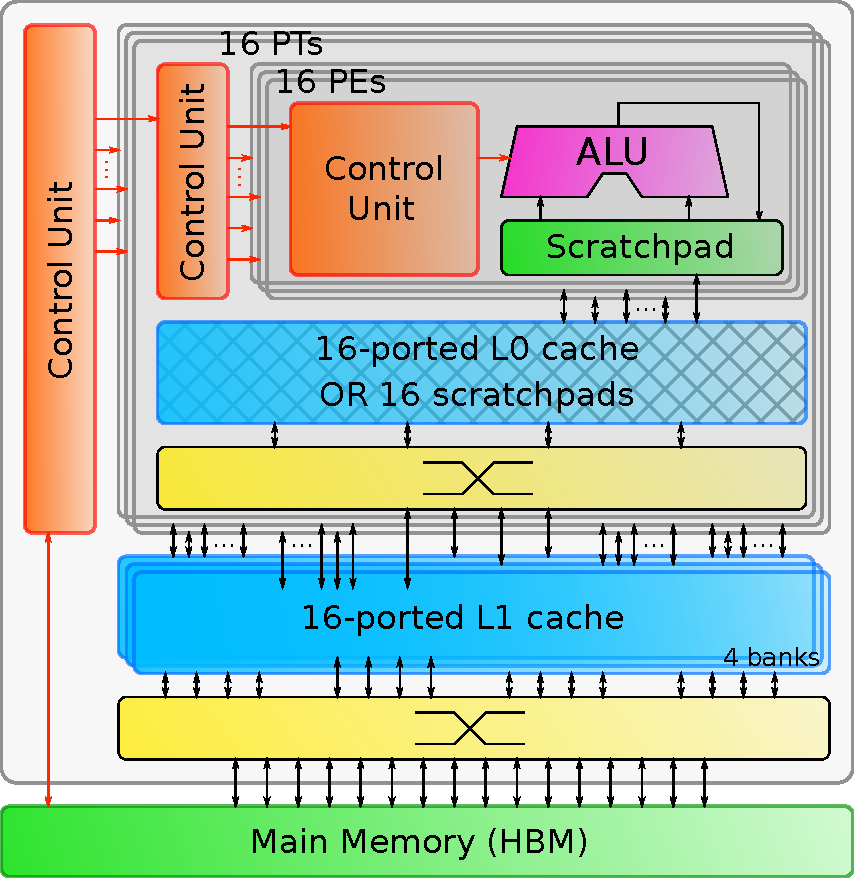
\includegraphics[width=0.7\textwidth]{Chapter_SoA/Figures/PDF/OuterSPACE.pdf}
            \caption{Architecture of OuterSPACE}
            \label{fig:soa:outerspace}
        \end{figure}
    \end{minipage}
    \hfill
    \begin{minipage}[b]{0.49\linewidth}
        \begin{figure}[H]
            \centering
            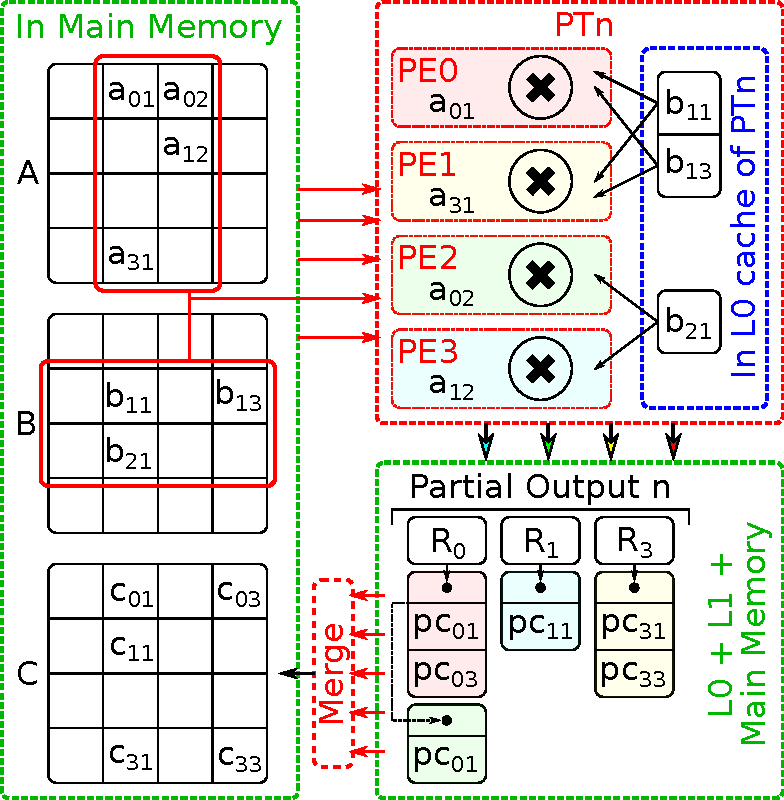
\includegraphics[width=0.705\textwidth]{Chapter_SoA/Figures/PDF/OuterSPACE_How_Vertical.pdf}
            \caption{OuterSPACE Data Flow}
            \label{fig:soa:outerspaceHow}
        \end{figure}
    \end{minipage}
\end{figure}

% %%%%%%%%%%%%%%%%%%%%%%%%%%%%%%%%%%%%%%%%%%%%%%%%%%%%%%%%%%%%%%%%%%%%%
% %% State-of-the-Art %%
% ExTensor
% %%%%%%%%%%%%%%%%%%%%%%%%%%%%%%%%%%%%%%%%%%%%%%%%%%%%%%%%%%%%%%%%%%%%%

\subsection{ExTensor}
\label{sec:soa:extensor}

The authors created ExTensor~\cite{Hegde2019_ExTensor} as a general purpose sparse tensor algebra accelerator (including SpMSpM). It is an \algo{OP} accelerator but due to its support for three levels of fixed \emph{tiling} of the inputs, it optimizes the \emph{intersection} search between non-zero elements or \emph{tiles}\footnote{Tensauraus~\cite{Srivastava2020_Tensaurus} is another accelerator designed for tensors, but their focus is on SpMM.}. By doing the \emph{intersections} ahead of time, at different levels of the memory hierarchy (which correspond to the \emph{tile} levels), ExTensor is able to efficiently eliminate \emph{ineffectual operations}, thus addressing the main issue in \algo{IP} or complex \emph{tiling} algorithms. Indeed, the input matrices would typically be stored in an \emph{(UOP, UOP, UOP, CP}) format, corresponding to three levels of \emph{tiling}.
ExTensor is designed with a flexible architecture composed of different bricks (see Figure~\ref{fig:soa:extensor}). To simply aid in the understanding, the interactions between the bricks are described using function calls:
\begin{itemize}
    \item The \emph{Scanner} is a storage unit that delivers a stream of coordinates in increasing order, fetching them from memory. The coordinates are delivered through the \emph{Iterate()} operation call.
    \item The \emph{Intersect} is a hardware block that co-iterates over several \emph{Scanners} in parallel and compares the coordinate streams. This unit performs the \emph{intersection} search required by \algo{IP} type algorithms, delivering a single stream with the matching coordinates, which are the coordinates of non-zero \emph{partial sums}. To optimise the \emph{intersection} step, it is possible to skip a range of coordinates in a stream depending on the current coordinate of another stream. Thus, the \emph{Intersect} sends skip messages with \emph{SkipTo()} operations to the other \emph{Scanners}.
    \item The \emph{Coordinator} is a hardware unit that includes \emph{Scanners} and \emph{Intersect} units, and manages the input and output data depending on the current processed \emph{tile}, as shown in Figure~\ref{fig:soa:extensor}. Data and \emph{metadata} are respectively stored in storage units and \emph{Scanners}, while a \emph{Sequencer} manages the \emph{Iterate()} calls so that the \emph{Intersect} brick delivers the stream of effective coordinates. In addition, in the \emph{Tile Coord} brick, the offsets of the \emph{tile} are added back, so the output of the \emph{Coordinator} is in absolute coordinates.
\end{itemize}

These bricks can be placed at different positions in a memory hierarchy, depending on the \emph{tiling} and selected hardware. Thus, the \emph{Coordinator} is able to intersect at coarse-granularity with output data being \emph{metadata} of the next \emph{tile}, skipping an entire \emph{tile} when appropriate, with low computation cost, and also at fine-granularity when output data are the non-zero elements that need to be multiplied.

ExTensor is designed with three levels of \emph{tiling} that each have  either input or output sequentiality. First, a \emph{Sequencer} plus \emph{Scanners} block~\ding{192} is placed close to the main memory to determine which \emph{tiles} to send to the next storage, the \emph{Last Level Buffer} (\emph{LLB}). Then, for each \emph{tile}, a \emph{Coordinator}~\ding{193} in the \emph{LLB} intersects the next level \emph{tiles}, which are sent to several \emph{PEs} that will process in parallel. Finally, in each \emph{PE}, a \emph{Coordinator}~\ding{194} intersects the non-zero elements of the computed \emph{tile} and sends them to the arithmetic unit of the \emph{PE} for multiplication.

In addition to these bricks which are the main contributions, ExTensor still needs to perform the \emph{merge} phase, including the \emph{reduction} of the \emph{POs} which are stored in \emph{CP$^{2}$} format. The \emph{Partial Output Buffer} (\emph{POB}), is managed by \emph{tiles}, and the content of the \emph{tile} is stored on-chip using a Content Addressable Memory (CAM) for quick access, enabling \emph{reductions} to be performed. On overflow, the \emph{tiles} are flushed to main memory. To benefit from ExTensor's support for \emph{tiling}, the input matrices need preprocessing, making it difficult to directly compare performance with other accelerators.

\begin{figure}
    \centering
    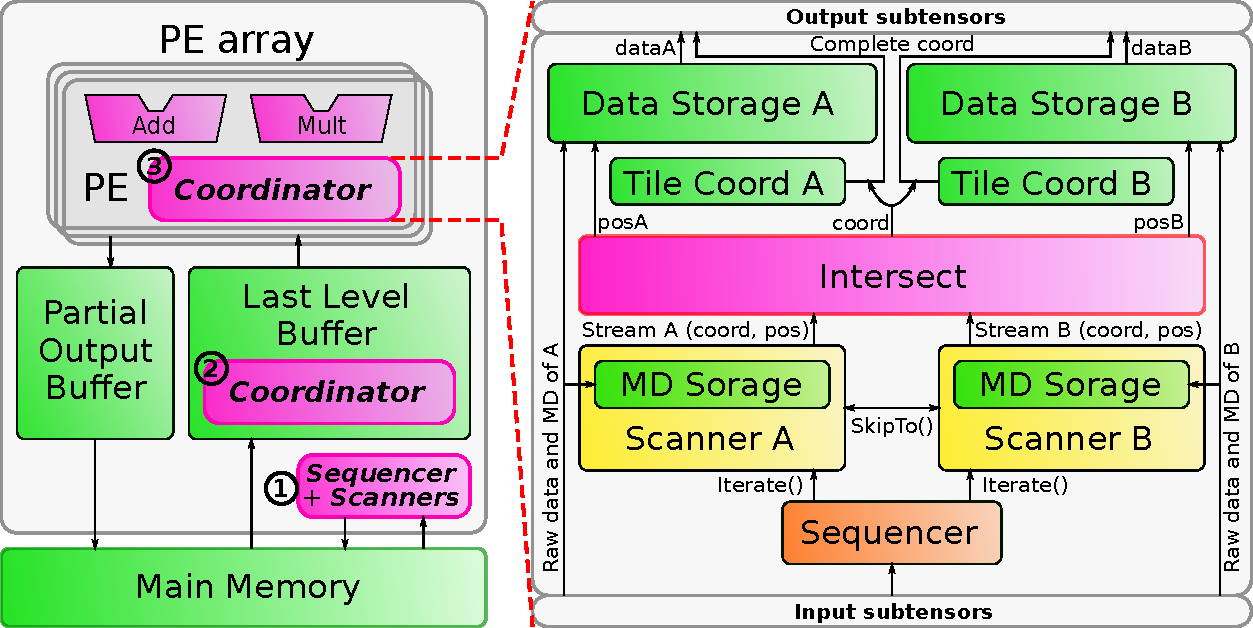
\includegraphics[width=0.6\linewidth]{Chapter_SoA/Figures/PDF/ExTensor.pdf}
    \caption{Architecture of ExTensor}
    \label{fig:soa:extensor}
\end{figure}

% %%%%%%%%%%%%%%%%%%%%%%%%%%%%%%%%%%%%%%%%%%%%%%%%%%%%%%%%%%%%%%%%%%%%%
% %% State-of-the-Art %%
% SpArch
% %%%%%%%%%%%%%%%%%%%%%%%%%%%%%%%%%%%%%%%%%%%%%%%%%%%%%%%%%%%%%%%%%%%%%

\subsection{SpArch}
\label{sec:soa:sparch}

SpArch~\cite{Zhekai2020_SpArch} uses an \algo{OP} algorithm for SpGEMM in order to benefit from the simplified access pattern for the inputs. To address the management of the large volume of \emph{POs}, SpArch  pipelines the \emph{multiply} and \emph{merge} phases and uses condensing methods to reduce the number of \emph{POs} and scheduling methods to reduce memory traffic.
Unlike other \algo{OP} accelerators~\cite{Pal2018_OuterSPACE}, with SpArch, both $A$ and $B$ are stored in \emph{(UOP, CP) row-major} format. As a consequence of this \emph{CSR} format, the $A$-rows can easily be condensed to the left (see Figure~\ref{fig:soa:sparch_algo}). Thus, when a condensed $A$-column is read, it will require reading all the $B$-rows corresponding to the different $A$-columns that have been combined. The \emph{MatA Column Fetcher} reads the combined $A$-columns and the \emph{MatB Row Prefetcher} reads the necessary $B$-rows (see Figure~\ref{fig:soa:sparch}), thus masking the memory latency. The \emph{MatB Row Prefetcher}, stores multiple $B$-rows in a cache, and it uses information about the upcoming $A$-columns  (provided by the \emph{Distance List Builder}) to ensure the needed $B$-rows are kept in the cache.

A key contribution of SpArch is the merge unit that is able to merge sixty-four \emph{POs} in parallel, through a binary tree type architecture. The core of the merger is a brick which compares and merges 4$\times$4 $(index, value)$ pairs in one cycle. These are combined to build a hierarchical merger array whose output is then written to main memory, and read back for further merging by the \emph{Partial Matrix Fetcher}. The authors note that the order in which the \emph{reductions} are performed is important, specifically sparser \emph{POs} should be merged first and they propose a Huffman tree scheduler to determine the best order to minimize memory accesses.
Overall, SpArch is able to compute an \algo{OP} SpGEMM\footnote{Since the merger can read \emph{POs} from memory, the $D$-matrix can be treated like an initial \emph{PO}.} kernel with reduced main memory traffic for the \emph{POs} mainly by addressing the \emph{scatter} problem with a highly parallelized merger.

\begin{figure}
    \centering
    \begin{minipage}[b]{0.54\linewidth}
        \begin{figure}[H]
            \centering
            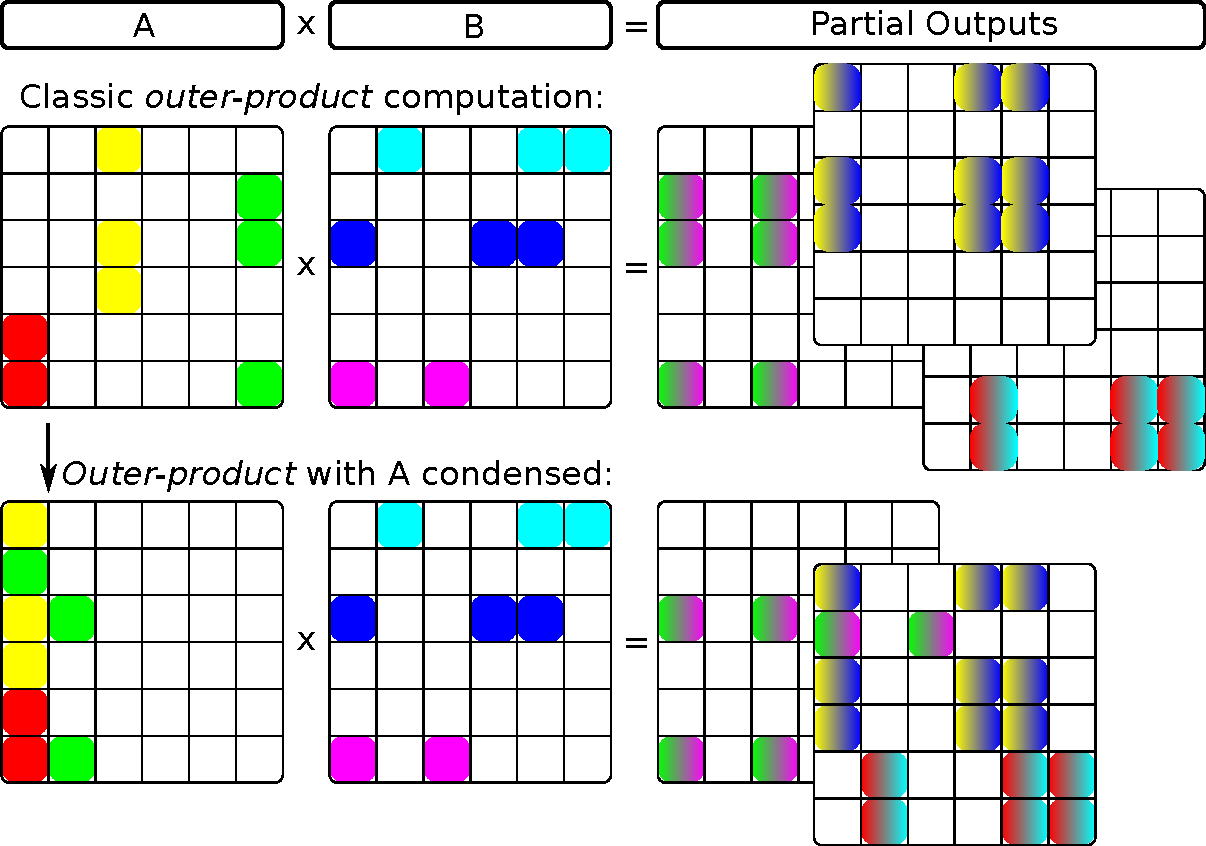
\includegraphics[width=0.85\linewidth]{Chapter_SoA/Figures/PDF/SpArch_algo.pdf}
            \caption{\emph{Outer-product} with a Condense $A$-Matrix}
            \label{fig:soa:sparch_algo}
        \end{figure}
    \end{minipage}
    \hfill
    \begin{minipage}[b]{0.44\linewidth}
        \begin{figure}[H]
            \centering
            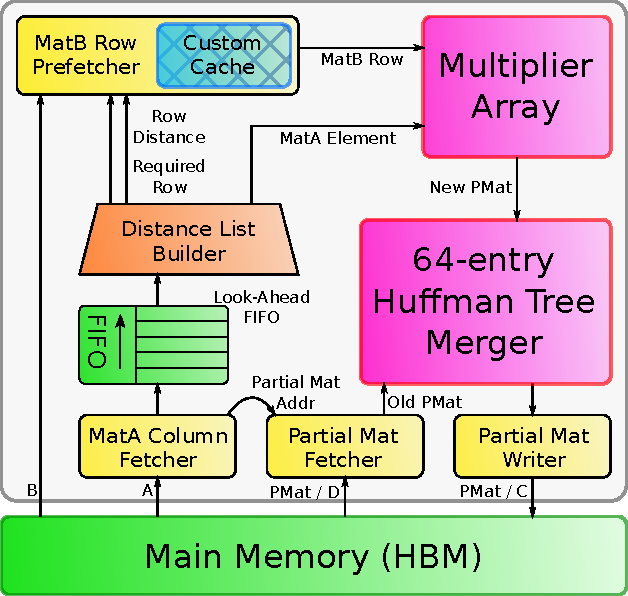
\includegraphics[width=0.8\linewidth]{Chapter_SoA/Figures/PDF/SpArch.pdf}
            \caption{Architecture of SpArch}
            \label{fig:soa:sparch}
        \end{figure}
    \end{minipage}
\end{figure}

% %%%%%%%%%%%%%%%%%%%%%%%%%%%%%%%%%%%%%%%%%%%%%%%%%%%%%%%%%%%%%%%%%%%%%
% %% State-of-the-Art %%
% MatRaptor
% %%%%%%%%%%%%%%%%%%%%%%%%%%%%%%%%%%%%%%%%%%%%%%%%%%%%%%%%%%%%%%%%%%%%%

\subsection{MatRaptor}
\label{sec:soa:matraptor}

MatRaptor~\cite{Srivastava2020_MatRaptor} is an accelerator designed to compute SpMSpM kernels. It is based on \algo{Gust} algorithm\footnote{Called \emph{row-wise product} in~\cite{Srivastava2020_MatRaptor}.}, which makes it possible to process multiple $A$-rows (2 to 8 for MatRaptor) in parallel. In MatRaptor (see Figure~\ref{fig:soa:matraptor}) a \emph{SpAL} (\emph{Sparse Matrix A Loader}) fetches non-zero elements of a $A$-row and sends them to a \emph{SpBL} (\emph{Sparse Matrix B Loader}). With the \emph{metadata} of this element, the \emph{SpBL} fetches non-zero elements of the corresponding $B$-rows and sends pairs of $A$- and $B$-elements to a \emph{PE}. This \emph{PE} computes the \emph{partial sums} and sends the results into queues for the \emph{merge} process. Instead of separating \emph{multiply} and \emph{merge} phases, several queues are used to store \emph{partial sums} and partially merged \emph{partial sums}, allowing the two phases to be pipelined. The \emph{PE} merges all the \emph{partial sums} resulting from an entire $A$-row, before sending the final output (the corresponding $C$-row) to main memory.

In MatRaptor, multiple $A$-rows are processed independently and in parallel in different \emph{PEs} and each \emph{PE} is assigned to a channel in an HBM memory~\cite{JESD235B}. It is important that each \emph{PE} can read its $A$-rows without interfering with the other \emph{PEs}. With the classic \emph{(UOP, CP) row-major} format, the rows are consecutive in memory and are not aligned to channel boundaries. To solve this problem, the authors propose a new format called \emph{C$^2$SR} (\emph{(FL, UOP, CP) channel-major}) that is based on a \emph{(UOP, CP) row-major}. For example, with two \emph{PEs}, all the elements of the even rows are stored in one channel, and the elements of the odd rows, in another channel, thus isolating the data. With this approach, the row pointers (\emph{UOP}) are no longer monotonic, which means that the length of a row can not be deduced by subtracting adjacent row pointers. This requires the addition of a new table (which we call \emph{fiber length} \emph{FL}), which stores the length of the non-zero elements in each row (see Figure~\ref{fig:soa:C2SR}). This modified storage format enables multiple \emph{PEs} to make effective use of the HBM.

MatRaptor is one of the first accelerators to use \algo{Gust} algorithm, however, it has some limitations regarding effective reuse of $B$-rows, both between parallel \emph{SpBLs} and temporally, as $A$ is traversed. A key contribution is the proposed \emph{C$^2$SR} input format, which makes it possible to separate rows into memory channels, to improve performance.

\begin{figure}
    \centering
    \begin{minipage}[b]{0.34\linewidth}
        \begin{figure}[H]
            \centering
            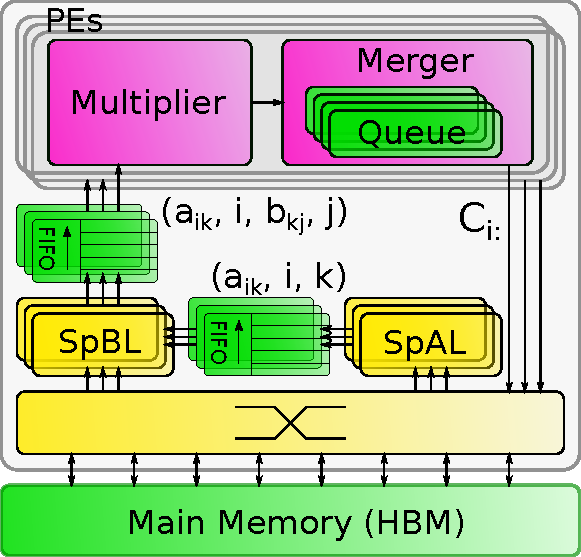
\includegraphics[width=0.85\textwidth]{Chapter_SoA/Figures/PDF/MatRaptor.pdf}
            \caption{Architecture of MatRaptor}
            \label{fig:soa:matraptor}
        \end{figure}
    \end{minipage}
    \hfill
    \begin{minipage}[b]{0.64\linewidth}
        \begin{figure}[H]
            \centering
            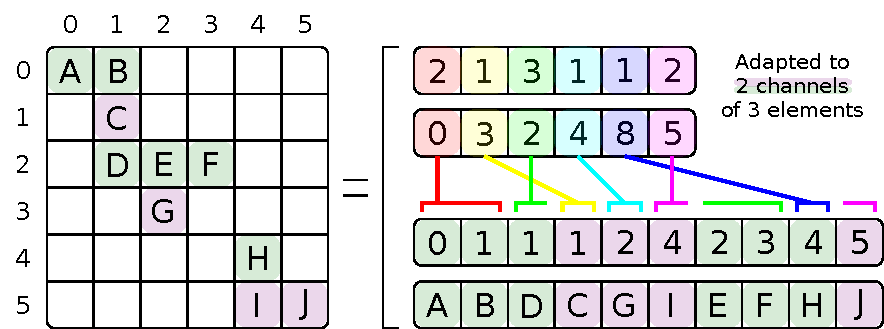
\includegraphics[width=0.9\textwidth]{Chapter_Background/Figures/PDF/SparseFormats/C2SR.pdf}
            \caption{\emph{(FL, UOP, CP) Channel-Major} Format ($C^{2}SR$)}
            \label{fig:soa:C2SR}
        \end{figure}
    \end{minipage}
\end{figure}

% %%%%%%%%%%%%%%%%%%%%%%%%%%%%%%%%%%%%%%%%%%%%%%%%%%%%%%%%%%%%%%%%%%%%%
% %% State-of-the-Art %%
% InnerSP
% %%%%%%%%%%%%%%%%%%%%%%%%%%%%%%%%%%%%%%%%%%%%%%%%%%%%%%%%%%%%%%%%%%%%%

\subsection{InnerSP}
\label{sec:soa:innersp}

InnerSP~\cite{Baek2021_InnerSP} is a SpMSpM accelerator based on the \algo{Gust} algorithm\footnote{The authors call this \emph{row-wise inner-product}, or confusingly sometimes \emph{inner-product}.}. The authors of InnerSP justify their choice by showing quantitatively that with the \algo{OP} the \emph{POs} represent a large volume of data, and that for many matrices the \emph{reductions} can not be done fully on-chip and thus must be buffered in main memory. Normally, with \algo{Gust} algorithm, $B$ must be read repeatedly, but InnerSP proposes a special cache for $B$ which exploits the spatial locality.

The architecture of InnerSP is shown in Figure~\ref{fig:soa:innersp}. The \emph{A reader} reads the $A$-rows. Two separate caches are used for $B$, one that stores the row pointers and the other which stores column indices and values. The \emph{B reader} reads the required $B$-rows, hopefully getting the data from the caches. Parallel multipliers perform the multiplications and then a hash-unit generates a hash based on the indices in $C$. A \emph{reduction} unit based on hash tables contains parallel comparators which search for matching hash values and performs the \emph {reductions}. When all the operations for a $A$-row are completed, the \emph{C writer} writes the $C$-row back to main memory.

% Figure located in Accelerators.tex

The architecture is efficient, as long as the \emph{Hash Reduction Unit} does not overflow. When overflows occur, the extra entries are temporarily stored in main memory, but there is a significant performance hit. To minimize the chance of overflows, InnerSP uses a pre-scanner to estimate the number of non-zero entries in the upcoming $C$-rows. The estimate primarily considers the $NNZ$ in the $A$-rows. If the estimated number of non-zero entries in $C$ exceeds the capacity of the \emph{Hash Reduction Unit}, then the row is split and processed in two passes. Conversely, if the number of non-zero entries in $C$ is small, two $A$-rows can be processed simultaneously.

To improve the performance of the $B$-cache, the authors exploit a technique from~\cite{Balaji2021_Popt}. The non-zero elements in the $A$-rows provide direct information about which $B$-rows are required. The column index table of $A$ is already pre-fetched by the \emph{A reader}, and when a row must be evicted from the $B$-cache, it chooses the ones which will not be required based on the upcoming entries in the column index table of $A$. This technique (also used by SpArch~\cite{Zhekai2020_SpArch}) maximizes the reuse of $B$-rows.

InnerSP is an accelerator based on \algo{Gust} algorithm which achieves high reuse of the $B$-rows, through a look-ahead in the $A$-\emph{metadata}.

\begin{figure}
    \centering
    \begin{minipage}[b]{0.54\linewidth}
        \begin{figure}[H]
            \centering
            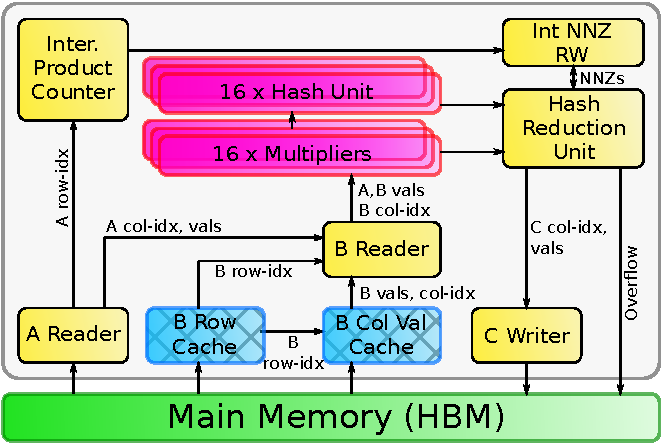
\includegraphics[width=0.9\textwidth]{Chapter_SoA/Figures/PDF/InnerSP.pdf}
            \caption{Architecture of InnerSP}
            \label{fig:soa:innersp}
        \end{figure}
    \end{minipage}
    \hfill
    \begin{minipage}[b]{0.44\linewidth}
        \begin{figure}[H]
            \centering
            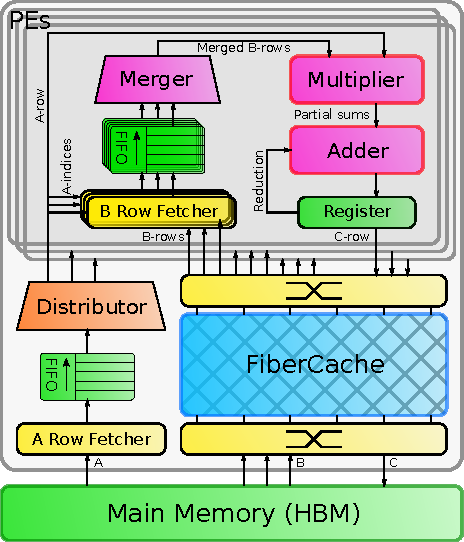
\includegraphics[width=0.8\textwidth]{Chapter_SoA/Figures/PDF/Gamma.pdf}
            \caption{Architecture of Gamma}
            \label{fig:soa:gamma}
        \end{figure}
    \end{minipage}
\end{figure}

% %%%%%%%%%%%%%%%%%%%%%%%%%%%%%%%%%%%%%%%%%%%%%%%%%%%%%%%%%%%%%%%%%%%%%
% %% State-of-the-Art %%
% Gamma
% %%%%%%%%%%%%%%%%%%%%%%%%%%%%%%%%%%%%%%%%%%%%%%%%%%%%%%%%%%%%%%%%%%%%%

\subsection{Gamma}
\label{sec:soa:gamma}

Gamma~\cite{Zhang2021_Gamma} is a dedicated accelerator for SpMSpM kernels, which uses \algo{Gust} algorithm. The two input matrices are both stored in \emph{(UOP, CP) row-major} format and the output is generated in the same format, providing consistency.

% Figure in Accelerators.tex

The Gamma architecture, presented in Figure~\ref{fig:soa:gamma}, is composed of a fetcher for the $A$-rows that contains a \emph{Distributor} to distribute them to 32 \emph{PEs}. Each \emph{PE} processes an entire $A$-row and computes the corresponding $C$-row. The \emph{PE} fetches the required $B$-rows and merges and sorts them in a 64-wide \emph{merge} block, before multiplying with the $A$-elements. As a result, the output $C$-row  is generated in order. The \emph{reduction} step is, thus, highly simplified, because any duplicate indices are adjacent. Normally, the $C$-row can be written back to main memory. However, if the $A$-row contains more than 64 non-zero elements, then it must be processed with multiple passes. After each pass, the partial $C$-row is stored temporarily. Finally, the temporary $C$-rows are read-back and merged by the \emph{PEs}.
Of course, the $B$-rows must be accessed repeatedly by the different \emph{PEs}, and Gamma proposes \emph{FiberCache} which is a highly banked cache which fetches the $B$-rows in advance, based on the column index table of $A$. It keeps track of which rows of $B$ are most needed by the \emph{PEs}, and when an eviction is necessary, the victim, is the row which is least needed.

Gamma encounters some difficulties when the $A$-matrix has rows that are too dense, requiring multiple iterations through the \emph{PEs}, which creates a high-load on the cache. The authors propose a software preprocessing technique which splits dense $A$-rows and rearranges them to make best use of the \emph{FiberCache}.

% Partial accelerators

% VL: SPiDRE and PHI here

% %%%%%%%%%%%%%%%%%%%%%%%%%%%%%%%%%%%%%%%%%%%%%%%%%%%%%%%%%%%%%%%%%%%%%
% %% State-of-the-Art %%
% SortCache
% %%%%%%%%%%%%%%%%%%%%%%%%%%%%%%%%%%%%%%%%%%%%%%%%%%%%%%%%%%%%%%%%%%%%%

\subsection{SortCache}
\label{sec:soa:sortcache}

The authors of SortCache~\cite{Srikanth2021_SortCache} note that modern processors are able to load an entire cache line in parallel but in many sparse applications less than 50\% of the data within a line is used, even with hand-tuned code. They propose a light SpGEMM accelerator which offloads the \emph{reduction} step, based on the \emph{Vectorized Binary Search Tree} (VBST), a data-structure from their earlier work~\cite{Srikanth2017_SuperStrider,Srikanth2019_MetaStrider}.
The VBST is a standard binary search tree where the size of node is a multiple of the cache block size and contains a sorted vector of $K$ $(key, value)$ pairs. Associated with each node is a \emph{pivot}; the pivots, with left and right child pointers, form a binary tree, as illustrated in Figure~\ref{fig:soa:sortcache_vbst}.

% Location of Figure in Accelerators.tex

Using the VBST, SortCache focuses on accelerating the \emph{scatter} updates to the output matrix, which are performed directly in the cache. The authors augment the processor with a single new instruction, \mbox{\emph{RED Key, Value}}. After $K$ updates have been issued, the hardware launches a \emph{reduction} in the SortCache, where the $K$ $(key, value)$ pairs are inserted into the VBST. This is done by traversing the tree from the root to the leaves. When duplicate keys are found, the \emph{reduction} operation is performed in the cache. When new keys are found, they are inserted, which can result in a temporary, new node with up to $2K$ $(key, value)$ pairs. This temporary node is partitioned, with one half having exactly $K$ entries. The insertion procedure may require visiting each level of the tree at least once ($\mathcal{O}(log(n)$) and it does not ensure the uniqueness of the keys, so at the end, an additional full traversal of the tree is required to remove duplicates.

The nodes closest to the root of the tree are accessed most frequently and are thus mapped to the caches closest to the processor. The authors propose to re-purpose cache tracking hardware (e.g. TAG values, LRU counters) to store the additional metadata (pivots, pointers). One of the difficulties with SortCache is that, in some cases, a large fraction of the VBST nodes are underutilized.

\begin{figure}
    \centering
    \begin{minipage}[b]{0.64\linewidth}
        \begin{figure}[H]
            \centering
            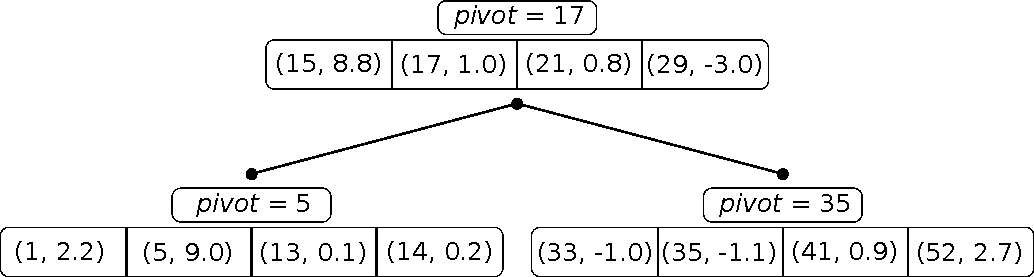
\includegraphics[width=\textwidth]{Chapter_SoA/Figures/PDF/VBST_example.pdf}
            \caption{VBST Data Structure Used by SortCache}
            \label{fig:soa:sortcache_vbst}
        \end{figure}
    \end{minipage}
    \hfill
    \begin{minipage}[b]{0.34\linewidth}
        \begin{figure}[H]
            \centering
            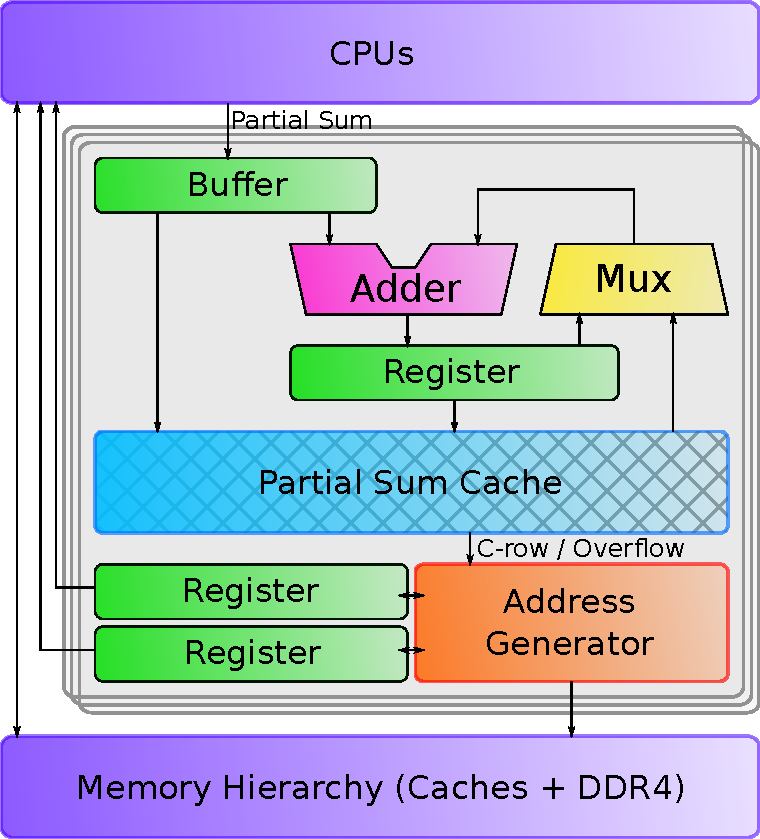
\includegraphics[width=\textwidth]{Chapter_SoA/Figures/PDF/ASA.pdf}
            \caption{Architecture of ASA}
            \label{fig:soa:asa}
        \end{figure}
    \end{minipage}
\end{figure}

% %%%%%%%%%%%%%%%%%%%%%%%%%%%%%%%%%%%%%%%%%%%%%%%%%%%%%%%%%%%%%%%%%%%%%
% %% State-of-the-Art %%
% ASA
% %%%%%%%%%%%%%%%%%%%%%%%%%%%%%%%%%%%%%%%%%%%%%%%%%%%%%%%%%%%%%%%%%%%%%

\subsection{ASA}
\label{sec:soa:asa}

In the scope of graph analytic problems, the authors of ASA~\cite{Zhang2022_ASA} observed that \algo{Gust} algorithm achieves high performance for SpGEMM kernels but note that it still requires acceleration for the \emph{reduction} step\footnote{The authors refer to the \emph{reduction} step as SPA (Sparse Accumulation).}. The software state-of-the-art for \emph{reduction} uses hash tables~\cite{Brock2021_GraphBLAS}. Some hardware accelerators, such as HTA~\cite{Zhang2019_HTA}, enhance performance for hash operations, but those solutions are not optimized for SpGEMM kernels. ASA is a low area, near-core extension for a general purpose processor that specifically accelerates the \emph{reduction} step for \algo{Gust} algorithm.

ASA accelerates \emph{reduction} operations received from software via custom instructions.
As presented in Figure~\ref{fig:soa:asa}, the \emph{partial sums} from these instructions are stored in a waiting buffer as $(index, value)$ pairs with a key that is a hash of the index, computed in software to maintain flexibility. The cache line, accessed with the key, is filled with the indices and the \emph{partial sums}. If a corresponding \emph{partial sum} is already stored, ASA accumulates it and writes back the result. If not, the \emph{partial sum} is simply stored into the cache. 

To minimize die area, the cache is not dimensioned for an entire $C$-row\footnote{The authors present a \emph{column-wise} \algo{Gust} implementation. This choice is arbitrary and, for consistency, we stick with a \emph{row-wise} presentation.} but ASA handles cache overflows in hardware. When a \emph{partial sum} needs to be stored in a fully filled cache line, a victim is selected and evicted, based on a LRU policy. The evicted entry is written into a pre-allocated FIFO queue in the memory hierarchy. ASA uses an address generator to manage evicted data and updates head and tail registers for the list. Software then traverses the list to merge duplicate keys to build the final output $C$-row. To avoid overflows, the authors advocate \emph{tiling} methods to efficiently distribute work through one or several ASA cores.

% Figure in Accelerators.tex

ASA is an accelerator which  optimizes the \emph{scatter} aspect of SpGEMM kernel with low area overhead, while leaving high software flexibility. Unlike other \algo{Gust} accelerators, there is no hardware \emph{gather} support for reusing or caching the $B$-rows.

%%%%%%%%%%%%%%%%%%%%%%%%%%%%%%%%%%%%%%%%%%%%%%%%%%%%%%%%%%%%%%%%
% Other Accelerators
%%%%%%%%%%%%%%%%%%%%%%%%%%%%%%%%%%%%%%%%%%%%%%%%%%%%%%%%%%%%%%%%
\subsection{Other Accelerators}
\label{sec:soa:other_accel}

In the above sections, we have described a selection of the main sparse accelerators that have appeared in the literature, covering different matrix multiplication algorithms and architectures. This list is not exhaustive, and in the following paragraphs we present several other accelerators which we will cover in less detail, due to space constraints.

\subsubsection{SPiDRE}

The authors of SPiDRE (Sparse Data Rearrange Engine)~\cite{Barredo2019_SPiDRE} propose a solution for the poor utilization of the memory hierarchy in sparse applications. They propose a near-memory data rearrangement engine. This engine can preprocess data, near memory, to create new data-structures that are dense and benefit from the memory hierarchy. For example, with a SpMV kernel, the input vector could be rearranged through a user defined function to a dense format where all non-zero elements are in the right order of computation.

\subsubsection{PHI}

The authors of PHI~\cite{Mukkara2019_PHI} note that many large graph algorithms favour pull (each node reads inputs from its neighbours) compared to push implementations (each node propagates results to its neighbours), as push implementations require read-modify-writes which require accessing complete cache lines, even though a small unit of data is modified. The authors include \algo{OP} SpMV (a push algorithm) in their evaluation.

PHI is a modified cache optimized to efficiently process commutative \emph{scatter} updates. When an update is received but the line is not in the cache, the line is not fetched, but rather marked as being in \emph{update mode}, where it simply stores the update. If subsequent updates hit the line, they are stored, or combined via the commutative operator. When a cache line is evicted, if it contains multiple updates, PHI assumes that the coalescing has been effective, and it processes the operations via a read-modify-write from main memory. If a cache contains few updates when evicted, PHI batches these updates as $(address, value)$ tuples, allocating a new cache line to assemble the batch. Groups of updates are organized by \emph{bins} corresponding to a small memory region. The batches are streamed to main memory. Later, the reading of the batches is also efficient, as they are contiguous.

In multi-core systems, private caches act as local buffers, thus coalescing the updates reduces coherency protocol traffic. This combination of in-cache coalescing and update buffering enables PHI to take advantage of locality when possible (like Coup~\cite{ZHANG_2015__Exploiting_Commutativity}), but with the addition of \emph{update batching}, PHI improves memory utilization, even when the data being updated is too large to fit in the cache.

\subsubsection{GSCSp}

GSCSp~\cite{LI_2023_GSCSp} is a FPGA-based accelerator based on \algo{Gust} algorithm. In other \algo{Gust} accelerators, a \emph{PE} processes a full $A$-row but the authors note that when there is variability in the number of elements in the $A$-rows, \emph{PEs} may be blocked, waiting for another \emph{PE} to complete. Thus the authors propose to distribute the elements in an $A$-row to different \emph{PEs} (\emph{element-wise} parallelism). Initially, each \emph{PE} buffers its output $C$-row, and when a \emph{PE} advances to the next row, it pushes its partial $C$-row to a final merger. The authors also propose to use separate caches for the \emph{metadata} for the $B$-rows and the values, and report that combined with the \emph{element-wise} parallelism, the approach is effective for reducing the memory traffic for accessing $B$-rows.

\subsubsection{Flexagon}

Flexagon~\cite{Munoz-Martinez2023_Flexagon} is a SpMSpM accelerator for DNN applications. The authors claim that the optimal algorithm (\algo{IP}, \algo{OP} and \algo{Gust}) depends on the matrix structure, potentially varying between DNN models and layers within a DNN, although in the majority of the cases, their data shows that \algo{Gust} is the most efficient. Flexagon is configurable: it can implement all three  algorithms. To achieve that, the authors designed a \emph{Merger-Reduction Network} (\emph{MRN}) that is able to perform multiplications (for \emph{partial sum} generation), accumulations (for \emph{reductions} operations) and comparisons (for \emph{intersection} searches and \emph{merge} phases) via a binary tree structure. Flexagon addresses the memory access issues of each algorithms via three custom memories: a FIFO for the $A$-matrix that is always read sequentially, a cache for the $B$-matrix that is subject to high temporal and spatial reuse in each of the three algorithms, and a PSRAM to store \emph{POs} for \algo{OP} and \algo{Gust} algorithms.

\subsubsection{Other Accelerators}

In GraphR~\cite{Song2018_GraphR}, the authors propose to use ReRAM technology and a cross-bar to perform graph operations directly in hardware, but this approach is not currently scalable to large problems. The ITS accelerator~\cite{Sadi2019_ITS} focuses on an \algo{OP} implementation of SpMV and they apply data-compression to the \emph{metadata}. The authors of SPU~\cite{Dadu2019_SPU} propose a more general hardware solution to input data dependencies and focus on graph applications. The focus of Alrescha~\cite{Asgari2020_Alrescha} is an innovative and adaptive preprocessing of the matrix in hardware to simplify the accesses to the $b$-vector. The authors of CoSparse~\cite{Feng2021_CoSPARSE} focus on a software layer that selects the hardware acceleration that is best adapted to the given problem.

The SSSR accelerator~\cite{Scheffler2023_SSSR} for RISC-V processors goes further by addressing \emph{intersection} and \emph{union} while streaming data to and from memory and it can be used for multiple kernels, however the RISC-V performance can not easily be compared with the other accelerators presented in this paper. In passing we note three other accelerators EIE~\cite{Han2016_EIE}, SCNN~\cite{Angshuman2017_SCNN} and CANDLES~\cite{Gudaparthi2022_CANDLES} which have hardware support for sparsity but which are highly focused on CNNs, besides SDMA~\cite{Gao2023_SDMA} that focuses on GNNs.

The SpaceA~\cite{Xie2021_SpaceA} accelerator exploits near-memory computing inside a 3D DRAM memory to implement SpMV using an \algo{IP} algorithm. With preprocessing, the rows of the matrix are assigned to banks within specific DRAM dies, while optimizing spatial locality. A separate die is used for storing the input and output vectors. Associated with each DRAM bank which stores the matrix, there is a \emph{PE} which reads the non-zero values of the matrix, fetches the required vector entries and performs the computations. Bringing the compute near the DRAM and exploiting emerging 3D technology, is an orthogonal approach to reduce memory access overheads.

\subsubsection{Other FPGA based Accelerators}

Many sparse accelerators have been prototyped on FPGAs~\cite{MOHAMMED_2022_SPARSE}. Indeed, AMD/Xilinx provide a turnkey library for SpMV~\cite{Xilinx_Vitis_2021, Li2023_OnXilinx}. In \cite{Du2022_HiSparse}, the authors propose a higher-performance SpMV using a modified \emph{CSR} format where the data is packed for efficient, streaming access in HBM\footnote{GraphLily~\cite{Hu2021_GraphLily} is a precursor of HiSparse, also from Cornell University.}. They also propose a highly-banked on-chip memory for the vector updates, and a hazard resolution strategy that allows efficient pipelining.

% %%%%%%%%%%%%%%%%%%%%%%%%%%%%%%%%%%%%%%%%%%%%%%%%%%%%%%%%%%%%%%%%%%%%%
% Comparison and Analysis
% %%%%%%%%%%%%%%%%%%%%%%%%%%%%%%%%%%%%%%%%%%%%%%%%%%%%%%%%%%%%%%%%%%%%%

\section{Comparison of Existing Accelerators}
\label{sec:soa:comparison_and_analysis}

In this section, we analyze and further compare the accelerators that were described in Section~\ref{sec:soa:hw_accelerators}. We start with Table~\ref{tab:soa:classificationMaturity} where we summarize the accelerators, chronologically, showing the research group where they were developed. We see that MIT is very active in the field, as they were involved in developing four different accelerators (\emph{e.g.} ExTensor, PHI, SpArch and Gamma).

\begin{table}
    \caption{Chronological Summary of Sparse Accelerators}
    \centering
    \footnotesize
    \begin{tabular}{|c|c|| >{\centering\arraybackslash}m{4.05cm}|| >{\centering\arraybackslash}m{7.19cm}|}
        \hhline{--||-||-}
        \textbf{Name} & \textbf{Date} & \textbf{Institute / University} & \textbf{Summary} \\
        \hhline{==::=::=}
        OuterSPACE~\cite{Pal2018_OuterSPACE} & 2018 & Univ. of Michigan / Arizona State Univ. & Highly parallelized SPMD, two levels cache -- \algo{OP} SpMSpM \\
        \hhline{--||-||-}
        ExTensor~\cite{Hegde2019_ExTensor} & 2019 & Univ. of Illinois / NVIDIA / MIT & General purpose tensor algebra -- With \emph{tiled} SpMSpM \\
        \hhline{--||-||-}
        PHI~\cite{Mukkara2019_PHI} & 2019 & MIT (CSAIL) / Carnegie Mellon Univ. & In cache, hash-based accelerator for \emph{reductions} \\
        \hhline{--||-||-}
        SPiDRE~\cite{Barredo2019_SPiDRE} & 2019 & UPC, BSC (Spain) / Arm Research & Near main memory data reorganisation for \emph{intersections} \\
        \hhline{--||-||-}
        MatRaptor~\cite{Srivastava2020_MatRaptor} & 2020 & Cornell & Row-parallel with HBM-aware custom format -- \algo{Gust} SpMSpM \\
        \hhline{--||-||-}
        SpArch~\cite{Zhekai2020_SpArch} & 2020 & MIT / Stanford / NVIDIA & Compression method to reduce \emph{POs}, \emph{multiply}/\emph{merge} pipe -- \algo{OP} SpGEMM \\
        \hhline{--||-||-}
        SpaceA~\cite{Xie2021_SpaceA} & 2021 & UC Santa Barbara & In memory accelerator for 3D DRAM -- \algo{IP} SpMV \\
        \hhline{--||-||-}
        Gamma~\cite{Zhang2021_Gamma} & 2021 & MIT (CSAIL) & Parallelized architecture with \emph{FiberCache} for $B$ -- \algo{Gust} SpMSpM \\
        \hhline{--||-||-}
        InnerSP~\cite{Baek2021_InnerSP} & 2021 & KAIST / DGIST (S. Korea) & $A$-look-ahead, caches for $B$, \emph{Hash Reduction Unit} for $C$ -- \algo{Gust} SpMSpM \\
        \hhline{--||-||-}
        SortCache~\cite{Srikanth2021_SortCache} & 2021 & Georgia Tech / Zettaflops / Sandia Labs & In cache accelerator for \emph{reductions}, based on the VBST \\
        \hhline{--||-||-}
        ASA~\cite{Zhang2022_ASA} & 2022 & Lehigh Univ. / Lawrence Berkeley & Custom cache accelerator for \emph{reductions} -- \algo{Gust} SpGEMM \\
        \hhline{--||-||-}
        Flexagon~\cite{Munoz-Martinez2023_Flexagon} & 2023 & Univ. of Murcia / Georgia Tech / NVIDIA & Configurable accelerator supporting all three algorithms -- SpMSpM \\
        \hhline{--||-||-}
        GSCSp~\cite{LI_2023_GSCSp} & 2023 & Nanyang Technological Univ. & Element-wise, FPGA-based accelerator -- \algo{Gust} SpMSpM \\
        \hhline{--||-||-}
    \end{tabular}
    \label{tab:soa:classificationMaturity}
\end{table}

\subsection{Benchmarks, Evaluation and Performance}

Up to this point, we have discussed the architecture of the various accelerators, without reporting the performance they achieve.
Most of the matrices used for benchmarking come from the SuiteSparse Matrix Collection~\cite{Kolodziej2019_SuiteSparse} that contains a large number of matrices from diverse, real applications. Domain specific matrix libraries are also used~\cite{Leskovec2014_SNAP, Smith2017_FROSTT, Azad2018_HipMCL, Reddi2020_MLPerf}, as well as some synthetic matrix generators~\cite{Ang2010_Graph500, Beamer2017_GAP}.
The densities are in general less than 1\% and can be as low as $10^{-5}$\%. ExTensor, SortCache and Flexagon also benchmark with denser matrices. In all cases, large matrices with several million $NNZ$, exceeding the size of a normal cache, have been evaluated.

\begin{table}
    \centering
    \caption{Qualitative Analysis and Evaluation of Sparse Accelerators}
    \footnotesize
    \begin{tabular}{|c|| >{\centering\arraybackslash}m{1.97cm}| >{\centering\arraybackslash}m{7.17cm}| >{\centering\arraybackslash}m{2.7cm}|}
        \hhline{-||---}
        \textbf{Name} & \textbf{Preprocessing\hyperlink{fn101}{$^{1}$}} & \textbf{Functional Evaluation (Tool / Evaluation Specifics / Host\hyperlink{fn102}{$^{2}$})} & \textbf{Local Memory Size} \\
        \hhline{=::===}
        OuterSPACE~\cite{Pal2018_OuterSPACE} & $A$ $\rightarrow$ \emph{row-major} & \emph{gem5} / Model only key elements; Skip memory allocation; Ignore start-up time / $\varnothing$ & 528KiB (33.8k entries) \\ % 1kB * 16 * 16 + 16kB * 16 + 4kB * 4 = 528kB -> 33ki elements (33.8k)
        \hhline{-||---}
        ExTensor~\cite{Hegde2019_ExTensor} & $A$, $B$ $\rightarrow$ highly \emph{tiled} custom format & Custom Python simulator / Only the \emph{Coordinator} is evaluated; Remainder modeled analytically / $\varnothing$ & $\sim$38MiB (2.5M entries) \\ % 64kB * 128 + 30MB + ? = ~ 38MB -> ~ 2.4Mi elements (2.5M)
        \hhline{-||---}
        PHI~\cite{Mukkara2019_PHI} & \emph{N/A} & \emph{ZSim} / Entirely evaluated / 16-cores system with 3 level cache & 32.3MiB (2.8M entries) \\ % 32kB + 256kB + 32MB = 32.3MB -> 2.7Mi elements (2.8M)
        \hhline{-||---}
        SPiDRE~\cite{Barredo2019_SPiDRE} & Not needed & \emph{gem5} / \emph{Unknown} / Single ARM core & $\varnothing$ (main memory size) \\ % no data but works in main memory
        \hhline{-||---}
        MatRaptor~\cite{Srivastava2020_MatRaptor} & $A$, $B$ $\rightarrow$ \emph{C$^2$SR} & \emph{gem5} / Entirely evaluated / $\varnothing$ & 320KiB (27.3k entries) \\ % 8 * 10 * 4KB = 320kB -> 26.7ki elements (27.3k)
        \hhline{-||---}
        SpArch~\cite{Zhekai2020_SpArch} & $A$, $B$ $\rightarrow$ \emph{row-major} & Custom C++ simulator / Entirely evaluated / $\varnothing$ & 940KiB (62.5k entries) \\ % 1024 * 12B + 1024 * 48 * 12B + 8192 * 12B + 16*16*16B(array) * 64 = 940kB -> 61ki element (62.5k)
        \hhline{-||---}
        SpaceA~\cite{Xie2021_SpaceA} & $A$ $\rightarrow$ row-aligned to DRAM banks & Custom simulator / Simulation tracking values stored in 3D-DRAM / $\varnothing$ & 4GiB (268.4M entries) \\ % 4GB -> 256Mi elements (268.4M)
        \hhline{-||---}
        Gamma~\cite{Zhang2021_Gamma} & $A$, $B$ $\rightarrow$ \emph{row-major} & Custom simulator / Entirely evaluated / $\varnothing$ & 3MiB (262.1k entries) \\ % 3MB -> 256ki elements (262,1k)
        \hhline{-||---}
        InnerSP~\cite{Baek2021_InnerSP} & Not needed & Custom simulator / Entirely evaluated / $\varnothing$ & $\leq$976.5KiB (119.9k entries) \\ % 4B * 1024 + 12B * 4096 + 8B * 1024 + 12B * 128 * 64 + 32kB (/8) + 256(or512)kB (/8) + 2 * 4B * 1024 + 16 * 16kB (/8) + 4B * 128 + 12B * 1024 = 720.5kB -> 85.1ki elements (87.2k) OR 976.5kB -> 117.1ki elements (119.9k)
        \hhline{-||---}
        SortCache~\cite{Srikanth2021_SortCache} & \emph{N/A} & Custom simulator / Entirely evaluated / Single threaded, in-order core  with 3 level cache & 16.3MiB (1.4M entries) \\ % 32kB + 256kB + 16MB = 16.3MB -> 1.4Mi elements (1.4M)
        \hhline{-||---}
        ASA~\cite{Zhang2022_ASA} & \emph{N/A} & Modified \emph{ZSim} / Entirely evaluated, one ASA per core / 8-cores with 3 level cache & 8$\times$8KiB (8$\times$1k entries) \\ % for one ASA: 8kB -> 1ki elements (1k)
        \hhline{-||---}
        Flexagon~\cite{Munoz-Martinez2023_Flexagon} & Not needed & Custom simulator based on STONNE / Entirely evaluated / $\varnothing$ & 1.3MiB (327.7k entries) \\ % open source soon // 256B + 1MB + 256KB (/4B) = 1.3MB -> 320.1ki elements (327.7k)
        \hhline{-||---}
        GSCSp~\cite{LI_2023_GSCSp} & $A$, $B$ $\rightarrow$ \emph{row-major} & HLS / FPGA Prototype / $\varnothing$ & 2.1MiB (178.2k entries) \\ % 40kB + 2MB = 2.1MB -> 174ki elements (178.2k)
        \hhline{-||---}
        \multicolumn{4}{l}{\hypertarget{fn101}{$^{1}$}We assume matrices are initially stored in \emph{(UOP, CP) column-major} format (\emph{CSC}).} \\
        \multicolumn{4}{l}{\hypertarget{fn102}{$^{2}$}Only for \emph{processor assist} accelerators.}
    \end{tabular}
    \label{tab:soa:evaluation}
\end{table}

% \begin{table}
%     \caption{Benchmark Matrices for Sparse MM and MV}
%     \begin{center}
%         \small
%         \begin{tabular}{|c||c|c|c|c|}
%             \hhline{-||----}
%             \textbf{Name} & \textbf{\# Matrices} & \textbf{Density Range} & \textbf{Largest NNZ} & \textbf{Sources} \\
%             \hhline{=::====}
%             \multirow{2}{*}{OuterSPACE~\cite{Pal2018_OuterSPACE}} & 20 & from 0.0001\% to 1.082\% & 16,518,948 & SuiteSparse and SNAP \\
%             \cline{2-5}
%             & \textit{unknown} & \textit{unknown} & \textit{unknown} & Graph500 R-MAT synthetic matrices \\
%             \hhline{-||----}
%             ExTensor~\cite{Hegde2019_ExTensor} & 14 & from 0.0002\% to 20.3\% & 11,524,432 & SuiteSparse and FROSTT \\
%             \hhline{-||----}
%             PHI~\cite{Mukkara2019_PHI} & 1 & 0.0001\% & 1,949,412,601 & SuiteSparse \\
%             \hhline{-||----}
%             SPiDRE~\cite{Barredo2019_SPiDRE} & \textit{unknown} & \textit{unknown} & \textit{unknown} & \textit{unknown} \\
%             \hhline{-||----}
%             MatRaptor~\cite{Srivastava2020_MatRaptor} & 14 & from 0.00061\% to 1.1\% & 5,105,039 & same as OuterSPACE \\
%             \hhline{-||----}
%             SpArch~\cite{Zhekai2020_SpArch} & 20 & from 0.0001\% to 1.082\% & 16,518,948 & same as OuterSPACE \\
%             \hhline{-||----}
%             SpaceA~\cite{Xie2021_SpaceA} & 15 & from 0.0003\% to 0.347\% & 14,148,858 & SuiteSparse \\
%             \hhline{-||----}
%             Gamma~\cite{Zhang2021_Gamma} & 37 & from 0.0001\% to 1\% & 16,518,948 & same as OuterSPACE plus SuiteSparse \\
%             \hhline{-||----}
%             \multirow{2}{*}{InnerSP~\cite{Baek2021_InnerSP}} & set of 755 & \textit{unknown} & 5,105,039 & SuiteSparse and SNAP \\
%             \cline{2-5}
%             & 14 & from 0.00061\% to 1.1\% & 5,105,039 & from OuterSPACE \\
%             \hhline{-||----}
%             SortCache~\cite{Srikanth2021_SortCache} & 11 & from 0.4\% to 78.5\% & 2,097,566 & SuiteSparse \\
%             \hhline{-||----}
%             ASA~\cite{Zhang2022_ASA} & 9 & from 0.00002\% to 0.3\% & $\sim$104,000,000 & HipMCL, SNAP and GAP \\
%             \hhline{-||----}
%             Flexagon~\cite{Munoz-Martinez2023_Flexagon} & 9 & from 6\% to 100\% & 2,718,144 & MLPerf \\
%             \hhline{-||----}
%             GSCSp~\cite{LI_2023_GSCSp} & 10 & from 0.09\% to 2.80\% & 484,256 & SuiteSparse \\
%             \hhline{-||----}
%         \end{tabular}
%         \label{tab:classificationMatrices}
%     \end{center}
% \end{table}

In Table~\ref{tab:soa:evaluation}, we note any required preprocessing, assuming, arbitrarily, that matrices are initially stored in \emph{CSC} format\footnote{This choice is based on the SuiteSparse Matrix Collection where matrices are stored \emph{column-major}.}. We see that a few accelerators require a conversion to their  specific format (\emph{e.g.} ExTensor and MatRaptor). PHI, SortCache and ASA are not concerned by preprocessing since they only address \emph{scatter}. In any case, fair benchmarking must take into account the cost of specialised preprocessing.

Not all accelerators have reached the same level of design maturity, and in Table~\ref{tab:soa:evaluation}, we have shown how each design was analyzed or simulated.
All designs report that they have been simulated at a cycle-accurate level. Most of the accelerators use custom simulators or tools like \emph{gem5}~\cite{Lowe2020_gem5}, \emph{ZSim}~\cite{SANCHEZ_2013_ZSIM} and STONNE~\cite{Munoz-Martinez2021_STONNE}, but unfortunately there is no common approach, making it difficult to fairly compare the reported performance. RTL descriptions are often only generated for key parts of the design. To estimate power and area, authors used tools such as CACTI~\cite{Balasubramonian2017_CACTI7} and McPAT~\cite{Li2009_McPAT}\footnote{We have not attempted to compare power/energy as the data in the literature is heterogeneous and can not be fairly compared.}.
In the last column of the table, we show the size of the local memory storage used in simulation by each accelerator. Except for SPiDRE and SpaceA which work directly in main memory, the local memories are in the range of 0.3MiB to 38MiB, corresponding to 27k to 2.8M entries. Thus, in the model presented in Section~\ref{sec:bg:AnalyticalModel}, most of the accelerators are situated in the middle-row of Figure~\ref{fig:bg:AnalyticalModel_SpMSpM}, with a local memory corresponding to a few matrix rows.

The accelerators performance are reported as a speedup versus a baseline, which may differ according to their hardware and software platforms: typically the Intel MKL library~\cite{Intel2003_IntelMKL} and the Armadillo library~\cite{Conrad2016_Armadillo} for CPUs, or cuSPARSE~\cite{NVIDIA2014_cuSPARSE} and CUSP~\cite{Dalton2014_Cusp} for GPUs.
Since different baselines with different numbers of threads and cores are used, these speedups need to be interpreted with care.
The speedups are in general higher for the \emph{standalone} accelerators as they provide optimized hardware for the entire kernel, while \emph{processor assist} accelerators have less impressive speedups but aim to be general purpose and have lower area overhead.

The only accelerators that have a comparable baseline are the \emph{standalone} ones addressing SpMSpM. They all compare themselves to OuterSPACE with the same benchmark matrices, so we can sort them by their speedup: Gamma ($6.6\times$)\footnote{This speedup increases to $7.7\times$ with their proposed preprocessing.}, InnerSP ($4.57\times$), SpArch ($4\times$), MatRaptor ($1.8\times$) and OuterSPACE ($1\times$).
Three of the five \emph{standalone} accelerators use the \algo{Gust} algorithm (Gamma, InnerSP and MatRaptor). SpArch, an \algo{OP} accelerator employing a complex architecture, outperforms MatRaptor, but does not achieve the same performance as InnerSP or Gamma, which suggests that \algo{Gust} is most adapted to high-performance hardware accelerators.

These measurements are consistent with our model presented in Section~\ref{sec:bg:AnalyticalModel} (Figure~\ref{fig:bg:AnalyticalModel_SpMSpM}). OuterSPACE, the baseline, corresponds to graph~\ding{196}. MatRaptor, the first \algo{Gust} accelerator, was able to achieve higher performance by reducing the number of \emph{random} accesses, and creating better regularity (red to yellow), as seen in graph~\ding{197}.

SpArch, is an \algo{OP} accelerator with a much larger local memory, which is used to address the red region in graph~\ding{196}. Their $A$-matrix condensing method, allows them to reduce the number of \emph{POs}, and approach the performance achievable in graph~\ding{199}, although, \emph{in fine}, it is impossible to store all the \emph{POs} in local memory. InnerSP and Gamma correspond to optimizations of the \algo{Gust} approach in graph~\ding{197}, to approach the performance in graph~\ding{200}. This is achieved by custom caches for the $B$-matrix to address the orange region. With the \algo{Gust} algorithm, it is only necessary to store a limited number of $B$-rows, which is achievable with the large local memories in these accelerators. The model presented in Section~\ref{sec:bg:AnalyticalModel} is helpful to understand the local memory requirements for SpMSpM accelerators.

%% RV %%
% \begin{table}
%     \caption{Reported Performance of Sparse Accelerators}
%     \begin{center}
%         \footnotesize
%         \begin{tabular}{|c|c|| >{\centering\arraybackslash}m{7cm} |c|c|c|}
%             \hhline{--||----}
%             & & \multicolumn{2}{c|}{\textbf{Baseline for Comparison}} & & \textbf{Average} \\
%             \cline{3-4}
%             \textbf{Name} & \textbf{Date} & \textbf{Hardware} & \textbf{Software} & \textbf{Kernels} & \textbf{Speedups} \\
%             \hhline{==::====}
%             %
%             \multirow{3}{*}{OuterSPACE} & \multirow{3}{*}{2018} & 6 cores/12 threads, 3.6 GHz Intel Xeon E5-1650V4 CPU & Intel MKL & \multirow{3}{*}{SpMV, SpMSpM} & \mbox{7.9$\times$} \\
%             \cline{3-4} \cline{6-6}
%             & & \multirow{2}{*}{NVIDIA Tesla K40 GPU} & cuSPARSE & & \mbox{1.13$\times$} \\
%             \cline{4-4} \cline{6-6}
%             & & & CUSP & & \mbox{1.14$\times$} \\
%             \hhline{==::====}
%             %
%             \multirow{2}{*}{ExTensor} & \multirow{2}{*}{2019} & \multirow{2}{*}{12 cores/24 threads, 3 GHz Intel Xeon E5-2687W v4 part} & \multirow{2}{*}{Intel MKL} & SpMSpM & \mbox{3.4$\times$} \\
%             \cline{5-6}
%             & & & & SpMM & \mbox{1.3$\times$} \\
%             \hhline{==::====}
%             %
%             \multirow{2}{*}{PHI} & \multirow{2}{*}{2019} & \multirow{2}{*}{2.2 GHz, 16 core x86-64 system} & outer-product & \multirow{2}{*}{SpMV} & \mbox{7$\times$} \\
%             \cline{4-4} \cline{6-6}
%             & & & inner-product & & \mbox{1.4$\times$} \\
%             \hhline{==::====}
%             %
%             SPiDRE & 2019 & single out-of-order Arm processor & \textit{unknown} & SpMV & \mbox{1.62$\times$} \\
%             \hhline{==::====}
%             %
%             \multirow{4}{*}{MatRaptor} & \multirow{4}{*}{2020} & single-threaded, 2.20 GHz Intel Xeon E5-2699 v4 server-class CPU & \multirow{2}{*}{Intel MKL} & \multirow{4}{*}{SpMSpM} & \mbox{77.5$\times$} \\
%             \cline{3-3} \cline{6-6}
%             & & 12 threads, 2.20 GHz Intel Xeon E5-2699 v4 server-class CPU & & & \mbox{7.9$\times$} \\
%             \cline{3-4} \cline{6-6}
%             & & NVIDIA Titan Xp GPU & cuSPARSE & & \mbox{37.6$\times$} \\
%             \cline{3-4} \cline{6-6}
%             & & OuterSPACE & $\varnothing$ & & \mbox{1.8$\times$} \\
%             \hhline{==::====}
%             %
%             \multirow{5}{*}{SpArch} & \multirow{5}{*}{2020} & 4-core ARM A53 CPU & Armadillo & \multirow{5}{*}{SpMSpM} & \mbox{1285$\times$} \\
%             \cline{3-4} \cline{6-6}
%             & & 6-core Intel Core-i7 5930K CPU & Intel MKL & & \mbox{19$\times$} \\
%             \cline{3-4} \cline{6-6}
%             & & \multirow{2}{*}{NVIDIA TITAN Xp GPU} & cuSPARSE & & \mbox{18$\times$} \\
%             \cline{4-4} \cline{6-6}
%             & & & CUSP & & \mbox{17$\times$} \\
%             \cline{3-4} \cline{6-6}
%             & & OuterSPACE & $\varnothing$ & & \mbox{4$\times$} \\
%             \hhline{==::====}
%             %
%             \multirow{3}{*}{Gamma} & \multirow{3}{*}{2021} & 4-core, 8-thread Skylake Xeon E3-1240 v5 & Intel MKL & \multirow{3}{*}{SpMSpM} & \mbox{33$\times$} \\
%             \cline{3-4} \cline{6-6}
%             & & OuterSPACE & \multirow{2}{*}{$\varnothing$} & & \mbox{6.6$\times$} \\
%             \cline{3-3} \cline{6-6}
%             & & SpArch & & & \mbox{1.84$\times$} \\
%             \hhline{==::====}
%             %
%             \multirow{4}{*}{InnerSP} & \multirow{4}{*}{2021} & 6-core Intel Core-i7 5930k CPU & Intel MKL & \multirow{4}{*}{SpMSpM} & \mbox{18.0$\times$} \\
%             \cline{3-4} \cline{6-6}
%             & & OuterSPACE & \multirow{3}{*}{$\varnothing$} & & \mbox{4.57$\times$} \\
%             \cline{3-3} \cline{6-6}
%             & & SpArch & & & \mbox{1.068$\times$} \\
%             \cline{3-3} \cline{6-6}
%             & & MatRaptor & & & \mbox{$2.45\times$} \\
%             \hhline{==::====}
%             %
%             SortCache & 2021 & single-threaded & \textit{unknown} & SpGEMM & \mbox{1.56$\times$} \\
%             \hhline{==::====}
%             %
%             \multirow{2}{*}{ASA} & \multirow{2}{*}{2022} & 8-core, 2.6 GHz architecture hash-based with main memory based on Micron MT40A2G4 and cache sizes and latency based on Intel i7-6700 & \textit{unknown} & \multirow{2}{*}{SpMSpM} & \mbox{2.25$\times$} \\
%             \cline{3-4} \cline{6-6}
%             & & HTA with similar cache sizes & $\varnothing$ & & \mbox{1.67$\times$} \\
%             \hhline{==::====}
%             %
%             GSCSp & 2023 & Xilinx Zynq UltraScale ZCU106 (quad-core ARM Cortex-A53) & row-wise & SpMSpM & \mbox{1.62$\times$} \\
%             \hhline{--||----}
%         \end{tabular}
%         \label{tab:classificationResults}
%     \end{center}
% \end{table}

%% RV %%
% (area * 14² / tech²) / 0.008 => norm_area (over PHI)
% \begin{table}
%     \caption{Main Memory Technology and Reported Die Area of Existing Accelerators}
%     \begin{center}
%         \begin{tabular}{|c|c||c|c|c||c|c|}
%             \hhline{--||---||--}
%             & & & & \textbf{Normalized} & \textbf{Main Memory} & \textbf{Main Memory} \\
%             \textbf{Name} & \textbf{Date} & \textbf{Technology ($nm$)} & \textbf{Area ($mm^2$)} & \textbf{Area} & \textbf{Technology} & \textbf{Bandwidth} \\
%             \hhline{==::===::==}
%             OuterSPACE & 2018 & 32 & 87 & 2081.54 & HBM2 & 128GB/s \\
%             \hhline{--||---||--}
%             ExTensor & 2019 & 32 & 96.89 & 2318.17 & \textit{unknown} & \textit{unknown}$^{\mathrm{1}}$ \\
%             \hhline{--||---||--}
%             PHI & 2019 & 14 & 0.008 & 1 (base) & DDR4 & 51.2GB/s \\
%             \hhline{--||---||--}
%             SPiDRE & 2019 & \textit{unknown} & \textit{unknown} & \textit{unknown} & \textit{unknown} & \textit{unknown} \\
%             \hhline{--||---||--}
%             MatRaptor & 2020 & 28 & 2.257 & 70.53 & HBM2 & 128GB/s \\
%             \hhline{--||---||--}
%             SpArch & 2020 & 40 & 28.49 & 436.25 & HBM2 & 128GB/s \\
%             \hhline{--||---||--}
%             Gamma & 2021 & 45 & 30.6 & 370.22 & HBM2 & 128GB/s \\
%             \hhline{--||---||--}
%             InnerSP & 2021 & 40 & 18.7 & 286.34 & HBM2 & 128GB/s \\
%             \hhline{--||---||--}
%             SortCache & 2021 & 15 & 0.79 & 86.02 & \textit{unknown} & \textit{unknown} \\ % in metastrider 128MB/s HBM
%             \hhline{--||---||--}
%             ASA & 2022 & 14 & 0.014 & 1.75 & DDR4 & 38.4GB/s \\
%             \hhline{--||---||--}
%             GSCSp & 2023 & \multicolumn{3}{c||}{ZCU106: $74\%$ LUTs / $47\%$ FFs / $\sim 60\%$ U-BRAM} & DDR4 & 6.4GB/s \\
%             \hhline{--||---||--}
%             \multicolumn{7}{l}{$^{\mathrm{1}}$The memory bandwidth is unknown but the CPU has a theoretical maximum bandwidth of 68.256GB/s.}
%         \end{tabular}
%         \label{tab:classificationArea}
%     \end{center}
% \end{table}

%%%%%%%%%%%%%%%%%%%%%EXTRA%INFOS%%%%%%%%%%%%%%%%%%%%%%
% OuterSPACE
% average throughput of 2.9 GFLOPS
% memory bandwidth utilization: 59.5-68.9\% for multiply phase and 46.5-64.8\% for merge phase

% SpArch
% memory bandwidth utilization: 68.6\%

% InnerSP
% --> 15.5 Glops, with 16 multipliers at 1~GHz.
%%%%%%%%%%%%%%%%%%%%%%%%%%%%%%%%%%%%%%%%%%%%%%%%%%%%%%

\subsection{Analysis for Designers}
\label{sec:soa:analysis}

\begin{figure}
    \centering
    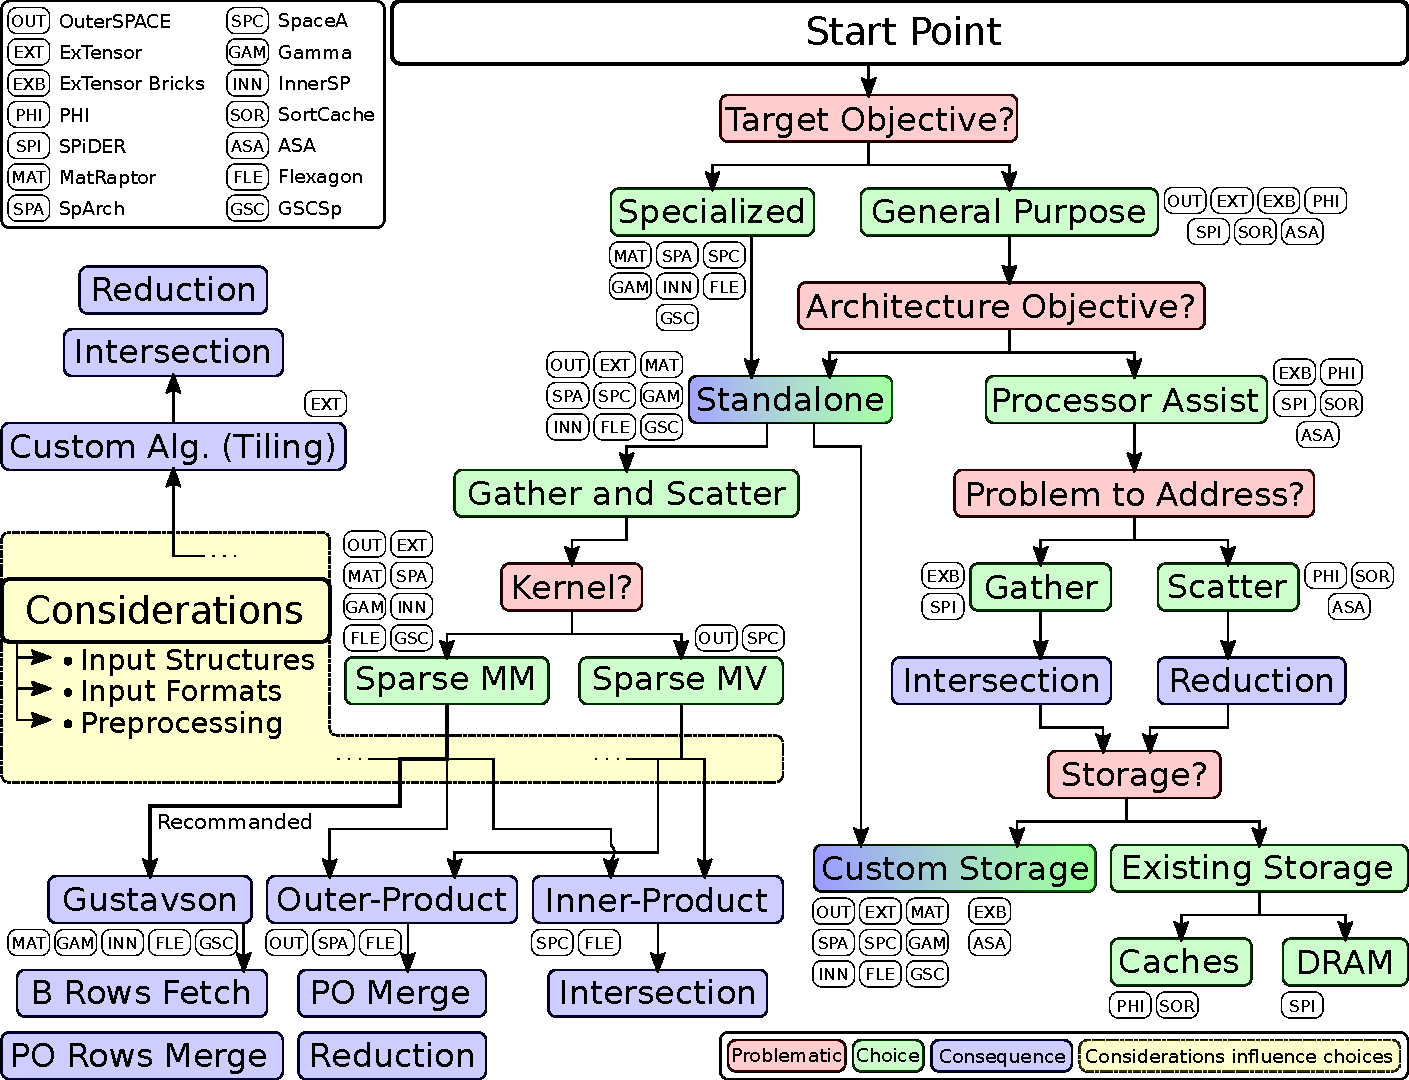
\includegraphics[width=\linewidth]{Chapter_SoA/Figures/PDF/Taxonomy.pdf}
    \caption{Flow Diagram for Architecture Selection}
    \label{fig:soa:taxonomy}
\end{figure}

There is no single "best overall" accelerator. A designer must consider the required performance, the available area and the class of problems to be addressed. In Figure~\ref{fig:soa:taxonomy} we present a flow diagram which can guide a designer towards an architecture based on their requirements. Starting from the top-right of the figure, the designer must first decide between a \emph{specialized accelerator} for a specific kernel or a \emph{general purpose accelerator}. The former is preferable if performance must be maximized, requiring a \emph{standalone} accelerator addressing both \emph{gather} and \emph{scatter} (\emph{e.g.} MatRaptor, SpArch, Gamma and InnerSP).

A \emph{general purpose accelerator} can either take the form of a highly configurable \emph{standalone} block (\emph{e.g.} OuterSPACE and ExTensor) or a \emph{processor assist} that boosts performance for a specific task. With a \emph{processor assist} (rightmost branch in the figure), the processor still performs important parts of the kernel, typically the multiplications, but off-loads the \emph{scatter} or \emph{gather} tasks to the accelerator, as these are the tasks which are the bottleneck with a traditional cache hierarchy. For example, for an \algo{IP} algorithm, the difficult part of the \emph{gather} task is performing the \emph{intersection} (e.g. the ExTensor bricks and SPiDRE).  Conversely, with \algo{OP} or \algo{Gust}, the challenge with the \emph{scatter} is to efficiently perform \emph{reductions} (e.g. PHI, SortCache and ASA). Finally, the designer must decide whether the storage is done by reusing existing memory resources (\emph{e.g.} PHI, SPiDRE and SortCache) or through custom caches/memories.

Going back to the case of a \emph{standalone} accelerator, the algorithms differ according to the supported kernels. For sparse MV, the accelerators studied here have opted for an \algo{OP} algorithm. For sparse MM, the designers of three of the five highest performing accelerators have chosen \algo{Gust} algorithm, as this algorithm provides a good trade-off, simplifying the \emph{gather} by reusing input $B$-rows and the row-by-row generation of the output, simplifying the \emph{scatter} aspect. The fact that the outputs are generated row-by-row, facilitates parallel implementations. \algo{Gust} works well with \emph{(UOP, CP)}, providing consistent input and output formats. Beyond the basic algorithm, \emph{tiling} approaches, as proposed by ExTensor, can be explored.

Orthogonal to previous choices, other design considerations are important. First, the starting point needs to be defined: some accelerators require software to perform \emph{tiling} (\emph{e.g.} ExTensor) or to rearrange the rows to improve performance (\emph{e.g.} Gamma). The cost of such preprocessing can be high, and is usually only justified if the same matrix is reused multiple times.

% %%%%%%%%%%%%%%%%%%%%%%%%%%%%%%%%%%%%%%%%%%%%%%%%%%%%%%%%%%%%%%%%%%%%%
% Conclusion 
% %%%%%%%%%%%%%%%%%%%%%%%%%%%%%%%%%%%%%%%%%%%%%%%%%%%%%%%%%%%%%%%%%%%%%

\section{Conclusion}
\label{sec:soa:conclusions}

% % Messages à passer
% \begin{itemize}
% \item Emerging field, increased activity
% \item Comparison of the SoA
% \item Memory hierarchy - not just a processing problem
% \item Gustavson
% \item Meta-data can be used to optimize caching strategies
% \item Innovative re-Use (re-purpose) of existing HW memory resources --> these accelerators can be integrated into existing memory systems
% \item Perhaps the key challenging is a highly parallelized reduction/merger
% \item None of the existing accelerators has focused on specific matrix structures
% \end{itemize}

The size of the datasets considered in computational physics, machine learning and graph analytics is continuing to grow and over the last six years, we note the emergence of many hardware accelerators designed to improve upon the performance of CPUs and GPUs. In this paper, we have presented the most important designs and established a comparison, while highlighting the underlying hardware challenges associated with sparse multiplication kernels.

As we have seen, with this class of problem, the challenge is to efficiently use the memory system despite the dereferencing required to access the \emph{metadata} associated with the \emph{sparse data formats}. Depending on the selected MM algorithm, the major challenge is either with the \emph{gather} and \emph{intersection} or with the \emph{scatter} updates. We have identified that accelerators based on \emph{Gustavson's} algorithm achieve a trade-off, where, on the \emph{gather} side, a limited number of $B$-rows need to be accessed, and on the output side, the result is generated row-by-row, simplifying the \emph{scatter} updates. The best \emph{Gustavson} accelerators have implemented further optimizations such as smart cache eviction strategies where the victim is selected by looking ahead at the $A$-indices. Several of the smaller \emph{processor assist} accelerators reuse existing cache memories and simply modify the behaviour of the control logic (directories, tags, eviction policies) to optimize the operation for sparse matrices. On the other hand, the highest performance accelerators propose dedicated, massively parallel \emph{reduction}/\emph{mergers}, to maximize parallelism.

Given the number and diversity of existing designs, it is clear that further hardware optimizations and improvements are possible. As stated earlier, there may never be a single "best" sparse accelerator, but rather designs that are best suited to specific classes of problems. We believe that the structure of the matrices is critical in terms of the sizing of caches and other resources, and that in the coming years, new accelerators will be increasingly tailored based on the structure of the matrices for specific classes of problems.

%%%%%%%%%%%%%%%%%

\clearpage